\section{Historical Background, Stylized Facts, and Empirical Results}
\label{sec:historical_empirical_results}
\label{sec:empirical_tournament}
\label{sec:empirical_results}

\subsection{Historical Background: The Rise of the Unidad Popular}
\label{sec:historical_background}
The Unidad Popular's electoral victory in 1970 brought a programme of socialist transformation into contact with social forces that had been reorganizing Chilean society for several decades. Industrial workers, rural laborers, \emph{pobladores}, students, and sections of the urban middle classes did not enter the political scene at the same moment or through the same institutions. Their demands were rooted in different locations of the economy and in different experiences of the developmental state. What gave the Popular Unity coalition its historical depth was the gradual convergence of conflicts around work, land, urban residence, and social rights. This section reconstructs that convergence as four waves of social conflict. Throughout, these historical waves must be distinguished from the accounting windows used in the empirical analysis: the waves describe historical political periods, whereas the profitability decompositions in Tables~\ref{tab:profitability_decomposition} and \ref{tab:accumulation_accounting} begin later and are bounded by annual data availability.

The economic background to these conflicts reaches back before the Great Depression. Chile entered the twentieth century as an export economy centered on nitrates, with mineral rents financing a large share of public revenue and sustaining commercial, fiscal, and urban expansion. This export boom also generated domestic demand. Public expenditure, mining settlements, transport networks, and the growth of Santiago, Valpara\'{\i}so, and other cities enlarged the market for locally produced manufactures. A meaningful manufacturing sector thus emerged well before state-led import substitution became an explicit development strategy. On the eve of the First World War, manufacturing represented roughly one-seventh of Chilean output, though concentrated primarily in food, beverages, textiles, clothing, and other simple consumer goods \citep{BulmerThomas2003}. This was industrial growth nested within an export economy rather than an autonomous industrial take-off.

In older historiography, the international disruptions beginning in 1914 were often treated as the decisive stimulus to domestic manufacturing \citep{Palma1984}. The newer reconstruction by P\'erez-Eyzaguirre substantially qualifies that interpretation. His revised series shows that Chilean industrial production had expanded alongside the export economy prior to 1914 and then contracted sharply when the war disrupted trade, imported inputs, and capital flows. Under this reconstruction, the level of industrial production achieved in 1913 was not recovered until 1941 \citep{PerezEyzaguirre2025}. The war exposed how strongly domestic manufacturing still depended on the commercial and financial circuits generated by primary exports, rather than initiating an uninterrupted wartime industrial boom.

Urbanization followed an equally distinctive trajectory. Chile was already highly urbanized by Latin American standards prior to the classic period of state-led industrialization. P\'erez-Eyzaguirre estimates that 46.7 percent of the population lived in urban settlements by 1930, emphasizing that the nineteenth- and early twentieth-century urban transition was tied more closely to export expansion, state formation, and successive primary-export cycles than to manufacturing employment alone \citep{PerezEyzaguirre2017}. This urban transition shaped subsequent labor politics: an urban population, an expanding state apparatus, and a domestic market formed before industry could absorb the majority of workers leaving rural activities. Chile entered the Depression with an unusually urban social structure relative to the productive apparatus supporting it.

The collapse after 1929 transformed these inherited tensions into a crisis of the existing accumulation pattern. Chile was among the Latin American economies most exposed to the contraction of world trade: the purchasing power of exports fell by roughly four-fifths during the first years of the Depression, while aggregate output fell dramatically between 1929 and 1932 \citep{BertolaOcampo2012,BulmerThomas2003}. Between 1929 and 1932, recorded employment fell from 1.43 million to 1.17 million workers, a loss of roughly 262,000 jobs, or 18 percent of the 1929 employment level. Over the same interval, measured unemployment increased from about 34,000 to 374,000 workers in the historical series used in this chapter, raising the unemployment rate from 2.35 to 24.30 percent. Beyond the immediate loss of national income, the collapse sharply contracted the foreign-exchange flows around which fiscal revenue, imports, mining demand, transport, commerce, and much of the domestic market had been organized. Restoring economic activity required a fundamentally different relation between the state, domestic demand, and production.

The initial policy response was pragmatic. Under Arturo Alessandri's second administration (1932--1938), deficit spending, public works, industrial credit, exchange controls, and tariff protection were deployed to reactivate employment and domestic production. As \citet{Silva2007} emphasizes, import substitution emerged during this stage through crisis management before crystallizing into a coherent developmental model. Emergency state intervention reorganized accumulation before the institutional machinery of the later developmental state was established. Industrial policy remained compatible with agrarian interests, supporting branches such as food processing and leather that were directly linked to domestic agriculture. This compatibility explains why early restructuring attracted joint support from financiers, merchants, landowners, and industrialists without requiring an immediate political rupture between an industrial bourgeoisie and a landed oligarchy.

Sources of growth between 1929 and 1939 reflect this structural redirection. For Chile over this decade, B\'ertola and Ocampo estimate that import substitution contributed approximately 1.3 percentage points per year to growth, while the contributions associated with domestic demand and exports were slightly negative, yielding aggregate output growth of only about 0.8 percent per year \citep{BertolaOcampo2012}. Domestic production substituted for imports while the external and domestic demand components inherited from the nitrate regime remained depressed. Manufacturing recovered much faster than aggregate activity, averaging roughly 7.7 percent annual growth between 1932 and 1939 \citep{BulmerThomas2003}---a trajectory of structural import substitution distinct from simple cyclical recovery.

The Popular Front victory in 1938 accelerated this transformation into a second stage. The creation of CORFO in 1939 provided the state with an institutional vehicle for economic planning, infrastructure provision, public enterprise, and the long-term financing of strategic industries. The expansion of electricity, steel, fuels, transport, and intermediate inputs widened the productive base beyond the light consumer branches inherited from the export era. Under CORFO's coordination, industry's share of GDP rose from approximately 13 percent in 1940 to roughly 21 percent in 1950 \citep{Silva2007}. During the Second World War, Chilean industrial output expanded much faster than aggregate GDP, consolidating manufacturing growth while world trade was disrupted \citep{BulmerThomas2003}. By 1950, manufacturing represented roughly a quarter of Chilean GDP in the B\'ertola--Ocampo estimates, exceeding the Latin American average \citep{BertolaOcampo2012}. The postwar economy was substantially more industrial than the economy that had entered the Great Depression.

The consolidation of Chilean import substitution coincided with the construction of what regulation theory identifies as Atlantic Fordism. In the United States and Western Europe, mass production was embedded in national growth regimes based on mass consumption, collective bargaining, Keynesian demand management, and welfare-state institutions, while Bretton Woods provided an international monetary framework compatible with national policy autonomy \citep{Vidal2015,Vidal2019}. Much of this Golden Age growth remained organized around domestic and regional mass markets rather than unrestricted global product-market competition.

The internationalization of this accumulation regime did not imply that peripheral economies reproduced the institutional architecture of the Fordist core. As \citet{Cardoso1972} emphasized in his analysis of the new forms of dependency, postwar foreign capital increasingly entered industrial production itself, often in combination with local private and state capital. Industrialization and structural dependency advanced together: while domestic manufacturing deepened, the reproduction of productive capacity remained asymmetrical because advanced technology and the production of means of production remained concentrated in the core capitalist economies. Dependent industrialization thus required external complementarity to complete its accumulation process, even as Latin America's share of world trade fell from 12 percent in 1948 to 6 percent in 1968 \citep{Cardoso1972}.

Chile's developmental trajectory was therefore a peripheral adaptation to the North Atlantic Fordist order rather than a domestic replica of Fordism. Industrial capacity expanded, but its reproduction deepened dependence on imported capital goods, intermediate inputs, replacement parts, foreign technology, and external finance. In his contemporary diagnosis of the early CORFO national accounts, \citet{Kaldor1959} observed that gross fixed-capital formation had only occasionally exceeded 10 percent of GNP after 1940, with more than half of domestic investment undertaken by the public sector. His estimates demonstrated that imported capital goods accounted for roughly two-fifths of fixed investment across the benchmark years examined. The external constraint had moved deeper into the production process itself.

Kaldor also identified an internal bottleneck central to Chilean accumulation: agriculture. Industrial output, non-agricultural employment, and urban incomes expanded faster than the domestic supply of food. Under these conditions, rising demand for wage goods exerted persistent upward pressure on food prices, which fed into wage demands and industrial operating costs. Kaldor treated agricultural stagnation, concentrated landholding, and low rural investment as an integral part of the same accumulation problem as industrial growth \citep{Kaldor1959}. The structural burden of sustaining basic infrastructure and capital formation fell disproportionately onto the state in the face of sluggish private domestic accumulation.

The social transformation generated by industrialization was decidedly uneven. Urbanization advanced faster than factory employment. Between 1940 and 1970, tertiary activities absorbed the largest share of net labor-force growth, while manufacturing and construction combined absorbed a considerably smaller share; the fact that positive sectoral contributions sum to more than 100 percent reflects the absolute contraction of primary-sector employment over the interval. By 1970, in an economically active population of about 3.2~million, \citet{DeVylder1976} counted roughly 260,000 openly unemployed workers and another 600,000 in low-productivity service activities. The city thus became the site where incomplete labor absorption, informal service employment, housing deficits, and unequal access to municipal infrastructure were systematically reproduced.

Chilean industrialization was disarticulated not because it failed to expand manufacturing, public employment, or basic infrastructure, but because productive capacity, labor absorption, and social incorporation proceeded at starkly uneven tempos. In 1970, 87.3 percent of rural dwellings and 26.8 percent of urban homes still lacked piped potable water \citep{DeVylder1976}. The state expanded education, healthcare, and social security while presiding over an unequal geography of incorporation. Migrants entered cities where social services and citizenship were materially more accessible than under the rural estate, even as stable factory employment and adequate housing remained scarce.

Rather than a rigid dichotomy between ``feudal'' estates and ``capitalist'' cities, the Central Valley hacienda had long combined commercial production for national and world markets with concentrated extra-economic control over tenant labor (\emph{inquilinaje}) \citep{Kay1980}. The gradual erosion of these agrarian relations released labor, altered the composition of the working class, and shifted the geographical terrain of collective mobilization without eliminating an urban labor reserve.

Four successive waves of social mobilization and state containment structured this developmental period. These waves track shifts in popular organization, the spatial locus of protest, and state responses. While macroeconomic profitability, capital accumulation, and employment bounded the material space in which disputes unfolded, political organization and state institutions decisively shaped how distributional pressures translated into collective action.

\begin{figure}[H]
\centering
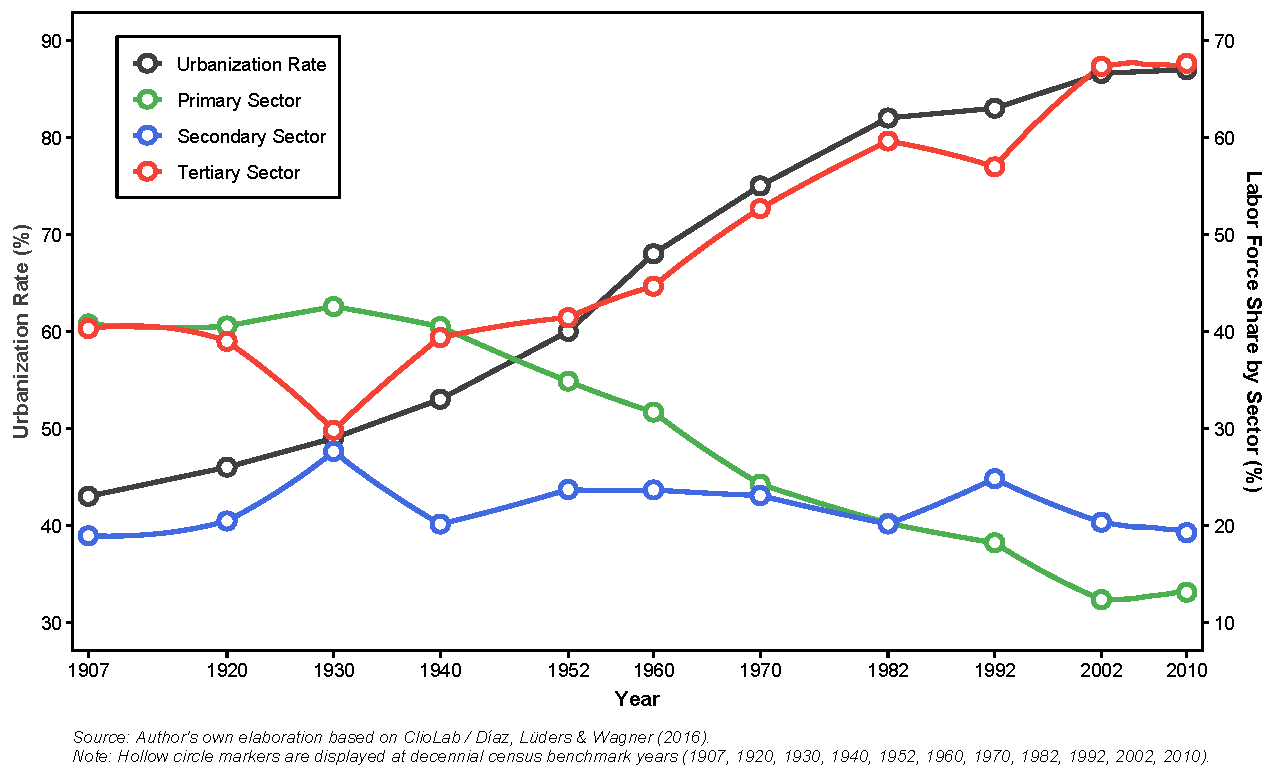
\includegraphics[width=0.90\textwidth]{figures/sec51/fig06_urbanization_labor_sectors.pdf}
\caption{Sectoral labor-force composition and urbanization in Chile, 1907--2010.}
\label{fig:sec51_urban_labor}
\begin{minipage}{0.90\textwidth}\footnotesize
\textit{Source:} Author's elaboration from Clio-Lab PUC historical statistics \citep{DiazLudersWagner2016}. Sectoral series refer to the labor force; urbanization refers to population. These measures have different denominators. Census urbanization observations are plotted as points.
\end{minipage}
\end{figure}

\paragraph{Wave I: Selective incorporation and coercive backlash, 1932--1947.}
The first wave emerged during the reconstruction of the 1930s and reached its crest in the mid-1940s. The 1931 Labor Code established a national framework for collective organization, but incorporation was highly uneven. Urban unions gained a recognized place in industrial relations and electoral politics, while agricultural workers remained subject to estate-level authority and legal restrictions \citep{Milos2008,Loveman1976}. The developmental state expanded productive and social capacities while preserving a differentiated labor regime between city and countryside.

This tension was visible from the beginning. The collapse of the export economy produced unemployment on a scale that weakened labor's immediate bargaining position, but it also destabilized established relations of authority. Rural workers and \emph{inquilinos} used petitions, strikes, and clandestine organization to demand statutory wages, written contracts, and security of tenure. The Ranquil conflict of 1934 exposed the coercive limits of incorporation in the countryside. Under the Popular Front, Communist and Socialist organizers intensified efforts to organize rural labor even as coalition governments remained cautious about confronting landowners directly \citep{Loveman1976}.

By the mid-1940s, rural mobilization converged with renewed industrial militancy. The Plaza Bulnes massacre and the general strikes of January and February 1946 marked the urban-industrial crest of this wave \citep{BravoVargas2017}. Registered agricultural petitions also rose sharply and reached their maximum in 1947 in the series assembled from Loveman's archival evidence (Figure~\ref{fig:sec51_petitions}). This is one reason the 1943--1947 profitability window in Table~\ref{tab:profitability_decomposition} should not be mistaken for the beginning of the wave: it captures the final observed segment of a conflict that had been building since the 1930s.

Distributional accounts are consistent with this tightening conflict. During 1943--1947, a declining profit share ($-5.53$ percent per annum) accounted for the primary negative contribution to profit-rate growth in the chapter's decomposition (Table~\ref{tab:profitability_decomposition}). While this pattern demonstrates that workers were gaining distributional ground in the observed interval, it reflects rather than explains the underlying political mobilization.

The state responded through legal segmentation and political repression. Law 8,811, enacted in July 1947, recognized agricultural unions while confining them to individual \emph{fundos}, restricting the seasonal timing of petitions, and imposing eligibility rules that blocked organization across estates \citep{Chile1947}. The following year, Law 8,987 outlawed the Communist Party and excluded targeted militants from electoral and union activity \citep{Chile1948}. These measures did not resolve rural grievances; they suppressed the organizational channels through which those grievances had been articulated.

The closure of rural organization altered the geography of conflict. Migration to urban centers was driven by structural factors predating the late 1940s repression, but the combination of agrarian stagnation, restricted rural organization, urban industrial concentration, and expanding municipal services made cities central to popular politics.

\begin{figure}[htbp]
\centering
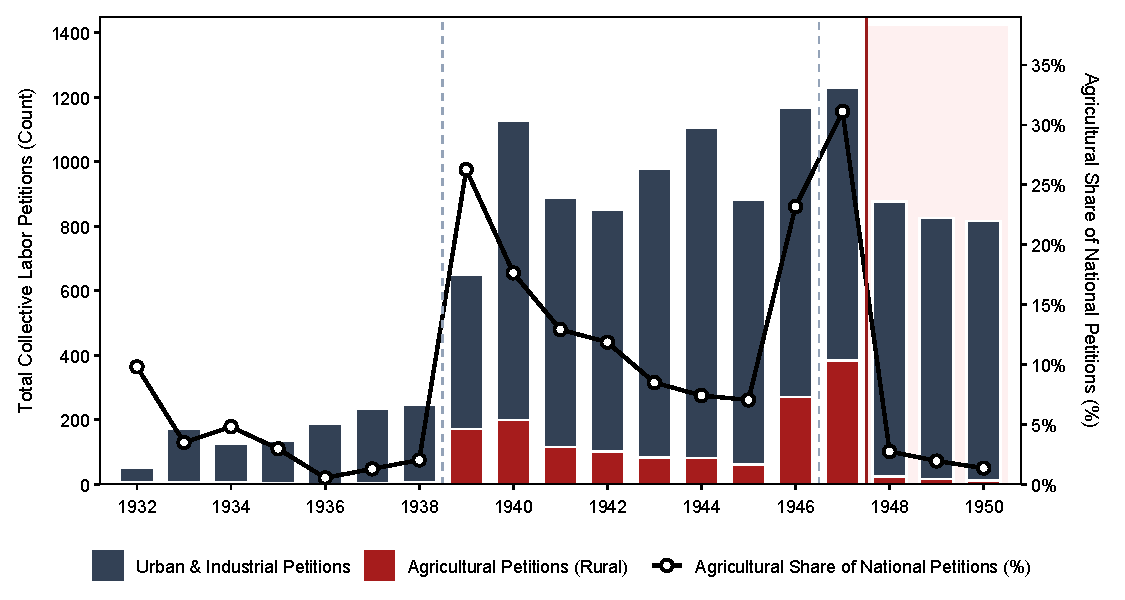
\includegraphics[width=0.88\textwidth]{figures/sec51/fig00_labor_petitions_composition_1932_1950.pdf}
\caption{Recorded collective labor petitions by sector, 1932--1950.}
\label{fig:sec51_petitions}
\begin{minipage}{0.88\textwidth}\footnotesize
\textit{Source:} Author's archival compilation from \citet{Loveman1976}. Petitions measure registered collective demands under the prevailing legal framework, not all forms of social conflict.
\end{minipage}
\end{figure}

\paragraph{Wave II: Coercive containment and urban recomposition, 1948--1958.}
The second wave was defined less by the disappearance of conflict than by its containment and relocation. The restrictions introduced in 1947--1948 narrowed legal space for rural and left organization. During the Ib\'a\~nez administration, the stabilization programme associated with the Klein--Saks mission added statutory wage restraint, credit contraction, and price increases on public transport and foodstuffs. Real wages fell sharply in the mid-1950s while inflation accelerated, shifting the costs of stabilization onto wage earners through workplace discipline and household consumption.

The profitability decomposition documents the distributional consequences of this containment. Between 1948 and 1958, a rising profit share ($+3.11$ percent per annum) provided the largest positive contribution to profit-rate growth ($+2.93$ percent per annum, Table~\ref{tab:profitability_decomposition}), while capital deepening ($-2.60$ log points) offset gains in potential labor productivity ($+2.29$ log points). Distribution shifted toward capital even as industrial and urban transformation continued.

Urban society, however, became more difficult to contain. Industrialization and public investment drew migrants toward the cities without providing factory employment or adequate housing on a commensurate scale. Rather than forming an inert residual of incomplete industrialization, urban neighborhoods became autonomous centers of collective action where migrants, factory workers, informal wage earners, and women organized around transport tariffs, food prices, housing, clinics, and municipal utilities.

In April 1957, protests over transit fare hikes erupted into a nationwide urban revolt, met by military suppression in Santiago, Valpara\'{\i}so, and Concepci\'on. In October 1957, organized families occupied land south of Santiago to establish the \emph{poblaci\'on} La Victoria. Pobladores did not merely petition the state for housing; they occupied land, organized settlement committees, constructed basic infrastructure, and negotiated collectively with public authorities \citep{Garces2002,Murphy2015}. While social conflict is sometimes characterized as having simply shifted from countryside to city, rural grievances persisted alongside industrial unionism and an emerging pobladores movement. What changed was the density of organizational ties linking these arenas.

\paragraph{Wave III: The Long Sixties and the rise of the Unidad Popular, 1959--1970.}
The Long Sixties transformed that urban and rural recomposition into a broader cycle of mobilization. Industrial workers expanded their demands beyond wages toward workplace control, challenging managerial authority over production quotas, safety, and the labor process. Inter-industry solidarity deepened through major conflicts, including the support of Huachipato steelworkers for the 1960 Lota coal strike, while state violence, such as the 1966 killings at the El Salvador copper mine, radicalized union federations \citep{Thielemann2018}.

In the countryside, the Agrarian Reform Law (Law 16,640) and the Rural Unionization Law (Law 16,625) enacted in 1967 dismantled the estate-bound restrictions of Law 8,811, recognizing communal unions and provincial confederations \citep{Chile1967}. Agricultural union membership expanded from 1,658 workers across 24 unions in 1964 to 127,680 members across 488 unions by mid-1970 \citep{DeVylder1976}. Across the economy as a whole, national union density over employed workers doubled from 11.2 percent in 1964 to 22.9 percent by 1970 \citep{OsorioPolanco2021} (Figure~\ref{fig:sec51_wageshare_unionization}). The organizational infrastructure of labor had become dense enough to coordinate action across sectors and regions.

Simultaneously, \emph{pobladores} expanded the politics of social reproduction beyond the wage relation. Land occupations, neighborhood committees, and demands for clinics, schools, transport, water, and paved roads turned access to the city into a field of collective bargaining with the state \citep{Garces2002,Murphy2015}. In centers such as Concepci\'on, industrial unions, student federations, and neighborhood assemblies coordinated strike support and shared logistical resources \citep{Schlotterbeck2018}. The popular movement supporting the Unidad Popular was an articulation of differentiated organized constituencies forged through the uneven development of the period.

Distributional mobilization unfolded within an expanding rather than a contracting economy: across the 1959--1970 accounting interval, the profit rate rose from 8.16 percent to 12.23 percent, supported by positive contributions from the profit share, capacity utilization, and potential labor productivity (Table~\ref{tab:profitability_decomposition}). Sustained accumulation, a larger urban labor force, and denser institutional networks expanded workers' capacity to press claims on national income, property, and state policy.

While a Kaleckian political mechanism links sustained high employment to weakened labor discipline, Chile had not attained generalized full employment. The sectoral and institutional dynamic was decisive: tighter conditions in unionized industries and rising national union density bolstered workers' collective bargaining power even while an informal reserve army persisted in peripheral services.

\begin{figure}[htbp]
\centering
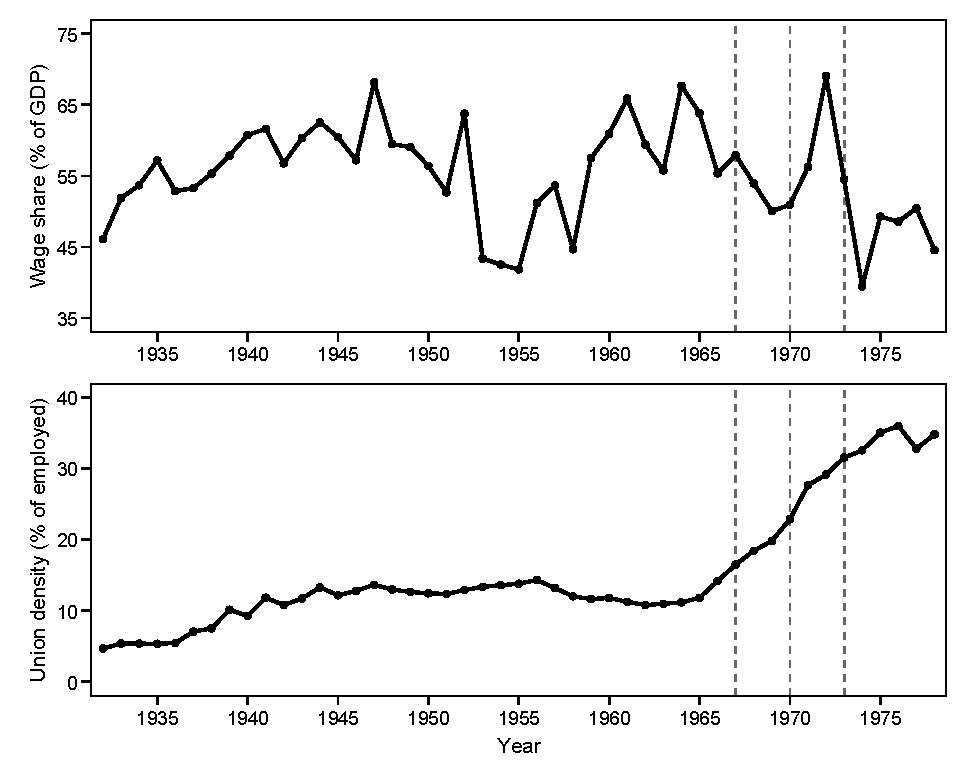
\includegraphics[width=0.88\textwidth]{figures/sec51/fig07_wageshare_unionization.pdf}
\caption{Wage share and unionization in Chile, 1932--1978.}
\label{fig:sec51_wageshare_unionization}
\begin{minipage}{0.88\textwidth}\footnotesize
\textit{Source:} Author's elaboration from \citet{Astorga2023} for Panel~A and \citet{OsorioPolanco2021} for Panel~B. Panel~A reports the functional wage share ($W/Y$, percent of GDP). Panel~B reports union density over employed workers. Vertical dashed lines mark the 1967 agrarian reform and rural unionization statutes (Laws 16,640 and 16,625), the September 1970 election of Salvador Allende, and the September 11, 1973 military coup.
\end{minipage}
\end{figure}

\paragraph{Wave IV: The UP administration and the crisis of accumulation, 1970--1973.}
Allende's election in September 1970 linked these popular movements directly with executive power. The UP programme connected income redistribution to the nationalization of strategic mineral resources, expansion of the social property area, agrarian expropriation, and structural planning. Yet the organizations forged during the preceding waves did not become passive extensions of government. Factory requisitions, land occupations, and community distribution networks frequently pushed ahead of the executive's statutory timetable \citep{Winn1986,Winn2016,Schlotterbeck2018}, generating dynamic tension between state policy and autonomous popular mobilization.

The administration's first year produced an exceptionally large distributive expansion. Real employee remuneration rose by 54.9 percent in 1971 following statutory wage adjustments \citep{DeVylder1976}, and the wage share rose from 50.9 percent of GDP in 1970 to 69.0 percent in 1972 \citep{Astorga2023}. The growth-accounting decomposition reveals a severe initial profit squeeze: the profit rate fell from 12.23 percent in 1970 to 6.57 percent in 1972, while the net accumulation rate declined from 4.23 to 1.85 percent and gross accumulation from 11.63 to 7.64 percent (Table~\ref{tab:accumulation_accounting}). The profit share accounted for most of this decline between 1971 and 1972 (Table~\ref{tab:profitability_decomposition}, Panel~B).

That initial distributive squeeze cannot be projected mechanically over the full three-year interval. Across 1971--1973, relative capital prices ($-4.35$ percent) and capacity utilization ($-4.78$ percent) provided the dominant negative contributions to profit-rate growth, while the contribution of the profit share changed sign (+1.94 percent, Table~\ref{tab:profitability_decomposition}, Panel~A). The annual accounts for 1973 make this divergence evident: the measured profit rate rebounded from 6.57 percent in 1972 to 9.12 percent in 1973, yet net capital accumulation slowed further to 1.71 percent (Table~\ref{tab:accumulation_accounting}). Because annual 1973 data aggregate the final eight months of the UP with the first four months of military dictatorship, they cannot separate pre-coup strikes from post-coup wage repression. They nevertheless demonstrate that profitability alone cannot explain the collapse of capital accumulation.

The terminal crisis concentrated contradictions that had accumulated across multiple decades: an industrial base dependent on imported capital goods and foreign finance; agrarian stagnation that generated wage-good bottlenecks; incomplete urban labor absorption; and a densely organized popular movement capable of mounting structural challenges to property and state authority.

The Unidad Popular concentrated rather than initiated these contradictions. Its redistributive programme accelerated popular mobilization within external and productive boundaries inherited from the developmental era. The next section examines the balance-of-payments constraints and monthly macroeconomic dynamics that governed the subsequent crisis.

\begin{table}[H]
	\centering
	\footnotesize
	\setlength{\tabcolsep}{3.8pt}
	\caption{Social Conflict Waves and Profitability Decomposition, Chile, 1943--1975}
	\label{tab:profitability_decomposition}
	
	\vspace{0.2em}

	
	\begin{tabular}{L{3.5cm}C{1.75cm}C{1.75cm}C{1.75cm}C{1.75cm}C{1.75cm}C{1.75cm}}
		\toprule
		\textbf{Wave of Social Conflict} 
		& \textbf{Profit Rate} 
		& \textbf{Profit Sh.} 
		& \textbf{Rel.\ Price} 
		& \textbf{Cap.\ Util.} 
		& \textbf{Lab.\ Prod.} 
		& \textbf{Cap.\ Deep.} \\
		
		& \small{$\Delta\ln r$} 
		& \small{$\Delta\ln(1-\omega)$} 
		& \scriptsize{$\Delta\ln(P_Y/P_K)$} 
		& \small{$\Delta\ln\mu$} 
		& \small{$\Delta\ln y^p$} 
		& \small{$-\Delta\ln k$} \\
		\midrule
		% Block 1: Regime Averages
		\multicolumn{7}{l}{\underline{\textit{A. Social Conflict Waves (Annualized Rates and \% Shares)}}} \\[0.3em]
		
		Wave I: Observed accounting segment (1943--1947)
		& \makecell[c]{-2.84\% \\ }
		& \makecell[c]{-5.53\% \\ (+194.9\%)}
		& \makecell[c]{+2.63\% \\ (-92.7\%)}
		& \makecell[c]{+0.62\% \\ (-21.7\%)}
		& \makecell[c]{-0.21\% \\ (+7.6\%)}
		& \makecell[c]{-0.34\% \\ (+11.9\%)} \\[0.5em]
		
		Wave II: Containment and urban recomposition (1948--1958)
		& \makecell[c]{+2.93\% \\ }
		& \makecell[c]{+3.11\% \\ (+106.1\%)}
		& \makecell[c]{-0.10\% \\ (-3.3\%)}
		& \makecell[c]{+0.23\% \\ (+7.9\%)}
		& \makecell[c]{+2.29\% \\ (+77.9\%)}
		& \makecell[c]{-2.60\% \\ (-88.6\%)} \\[0.5em]
		
		Wave III: Long Sixties accounting interval (1959--1970)
		& \makecell[c]{+2.07\% \\ }
		& \makecell[c]{+1.31\% \\ (+63.3\%)}
		& \makecell[c]{+0.45\% \\ (+21.6\%)}
		& \makecell[c]{+0.97\% \\ (+46.9\%)}
		& \makecell[c]{+1.72\% \\ (+83.0\%)}
		& \makecell[c]{-2.38\% \\ (-114.8\%)} \\[0.5em]
		
		Wave IV: UP crisis accounting interval (1971--1973)
		& \makecell[c]{-7.65\%\\  }
		& \makecell[c]{+1.94\% \\ (-25.3\%)}
		& \makecell[c]{-4.35\% \\ (+56.9\%)}
		& \makecell[c]{-4.78\% \\ (+62.5\%)}
		& \makecell[c]{-1.23\% \\ (+16.0\%)}
		& \makecell[c]{+0.77\% \\ (-10.1\%)} \\[0.8em]
		
		\midrule
		
		% Block 2: Annual Crisis Cycle
		\multicolumn{7}{l}{\underline{\textit{B. Terminal Crisis Cycle: Annual Log Changes and \% Shares}}} \\[0.3em]
		
		$1970 \to 1971$: Reactivation peak 
		& \makecell[c]{-14.05\% \\ }
		& \makecell[c]{-11.44\% \\  (+81.4\%)}
		& \makecell[c]{-7.90\% \\ (+56.2\%)}
		& \makecell[c]{+5.92\% \\ (-42.1\%)}
		& \makecell[c]{-0.43\% \\ (+3.1\%)}
		& \makecell[c]{-0.20\% \\ (+1.4\%)} \\[0.5em]
		
		$1971 \to 1972$: Profit squeeze 
		& \makecell[c]{-48.08\% \\ }
 		& \makecell[c]{-34.60\% \\ (+72.0\%)}
		& \makecell[c]{-10.42\% \\ (+21.7\%)}
		& \makecell[c]{-2.52\% \\ (+5.2\%)}
		& \makecell[c]{-2.27\% \\ (+4.7\%)}
		& \makecell[c]{+1.74\% \\ (-3.6\%)} \\[0.5em]
		
		$1972 \to 1973$: Annual observation spanning the coup 
		& \makecell[c]{+32.78\% \\ }
		& \makecell[c]{+38.48\% \\ (+117.4\%)}
		& \makecell[c]{+1.72\% \\ (+5.3\%)}
		& \makecell[c]{-7.04\% \\ (-21.5\%)}
		& \makecell[c]{-0.18\% \\ (-0.5\%)}
		& \makecell[c]{-0.20\% \\ (-0.6\%)} \\[0.5em]
		
		$1973 \to 1974$: DL 522 compression 
		& \makecell[c]{+15.74\%}
		& \makecell[c]{+28.59\% \\ {\scriptsize (+181.7\%)}}
		& \makecell[c]{-11.47\% \\ {\scriptsize (-72.9\%)}}
		& \makecell[c]{-0.72\% \\ {\scriptsize (-4.6\%)}}
		& \makecell[c]{+4.04\% \\ {\scriptsize (+25.7\%)}}
		& \makecell[c]{-4.70\% \\ {\scriptsize (-29.9\%)}} \\[0.5em]
		
		$1974 \to 1975$: Chicago shock therapy 
		& \makecell[c]{-48.97\%}
		& \makecell[c]{-17.70\% \\  (+36.2\%)}
		& \makecell[c]{-16.24\% \\ (+33.2\%)}
		& \makecell[c]{-14.78\% \\ (+30.2\%)}
		& \makecell[c]{+8.97\% \\ (-18.3\%)}
		& \makecell[c]{-9.22\% \\ (+18.8\%)} \\
		\bottomrule
	\end{tabular}%
	
	\vspace{0.5em}
	
	\begin{minipage}{\textwidth}
		\scriptsize
		\textit{Notes.} Growth-accounting decomposition using the identity $\Delta \ln r_t \equiv \Delta \ln(1-\omega_t) + \Delta \ln(P_{Y,t}/P_{K,t}) + \Delta \ln \mu_t + \Delta \ln y^p_t - \Delta \ln k_t$. Values outside parentheses are annualized log contributions (\% p.a.). Values inside parentheses report the component's share of the total change, computed as $(\Delta \ln X_i / \Delta \ln r_t) \times 100\%$. A positive share indicates the component moved in the same direction as the total change; a negative share indicates it offset the total change. Shares may exceed 100\% due to normalization by the net total change. Source: Author's own elaboration (Chapter 2).
	\end{minipage}
\end{table}

\begin{table}[H]
	\centering
	\footnotesize % Matched to Table 1
	\setlength{\tabcolsep}{4pt}
	
	\caption{Capital Accumulation Response Across the Terminal Crisis Cycle, Chile, 1964--1975}
	\label{tab:accumulation_accounting}
	
	\vspace{0.2em}
	
	% Reuse the custom column types defined in Table 1's preamble 
	% OR define them here if they are local. 
	% Assuming L{} and C{} are already defined globally in your preamble:
	
	% Total Width Calculation to match Table 1:
	% Table 1: 3.5 + (6 * 1.75) = 3.5 + 10.5 = 14.0 cm
	% Table 2: 3.5 + (5 * X) = 14.0 => 5X = 10.5 => X = 2.1 cm
	% So we use C{2.1cm} for the numeric columns.
	
	\begin{tabular}{L{3.5cm} C{2.1cm} C{2.1cm} C{2.1cm} C{2.1cm} C{2.1cm}}
		\toprule
		\textbf{Episode / Year} 
		& \textbf{Profit Rate} 
		& \textbf{Accum.\ Ratio} 
		& \textbf{Gross Acc.\ Rate} 
		& \textbf{Depreciation Rate} 
		& \textbf{Net Acc.\ Rate} \\
		
		& $\boldsymbol{r}$ (\%) 
		& $\boldsymbol{\chi}$ (ratio) 
		& $g^{\mathrm{gross}}_K$ (\%) 
		& $\boldsymbol{\delta}$ (\%) 
		& $g^n_K$ (\%) \\
		\midrule
		
		\multicolumn{6}{l}{\underline{\textit{A. Christian Democratic Administration (1964--1970)}}} \\[0.3em]
		
		1964 (Baseline)       & 8.16  & 1.530 & 12.49 & 7.67 & 4.82 \\[0.2em]
		1965                  & 8.59  & 1.244 & 10.69 & 6.94 & 3.75 \\[0.2em]
		1966                  & 10.94 & 0.972 & 10.63 & 6.97 & 3.66 \\[0.2em]
		1967                  & 10.14 & 1.066 & 10.81 & 7.06 & 3.75 \\[0.2em]
		1968                  & 11.29 & 0.991 & 11.20 & 7.24 & 3.96 \\[0.2em]
		1969 (Peak Profit.)   & 12.79 & 0.857 & 10.96 & 7.14 & 3.82 \\[0.2em]
		1970 (Inherited)      & 12.23 & 0.951 & 11.63 & 7.40 & 4.23 \\[0.5em]
		
		\midrule
		
		\multicolumn{6}{l}{\underline{\textit{B. Unidad Popular Administration (1971--1973)}}} \\[0.3em]
		
		1971 (Reactivation)   & 10.62 & 0.953 & 10.12 & 6.78 & 3.34 \\[0.2em]
		1972 (Squeeze)        & 6.57  & 1.162 & 7.64  & 5.78 & 1.85 \\[0.2em]
		1973 (Coup year)      & 9.12  & 0.821 & 7.48  & 5.78 & 1.71 \\[0.5em]
		
		\midrule
		
		\multicolumn{6}{l}{\underline{\textit{C. Military Dictatorship \& Shock Therapy (1974--1975)}}} \\[0.3em]
		
		1974 (Compression)    & 10.67 & 0.811 & 8.65  & 6.27 & 2.38 \\[0.2em]
		1975 (Collapse)       & 6.54  & 1.035 & 6.77  & 5.56 & 1.21 \\
		
		\bottomrule
	\end{tabular}%
	
	\vspace{0.5em}
	
	\begin{minipage}{\textwidth}
		\scriptsize
		\textit{Notes.} Accumulation accounting for fixed capital assets ($K_t \equiv K_{\mathrm{ME},t} + K_{\mathrm{NRC},t}$), excluding residential construction. Gross accumulation is $g^{\mathrm{gross}}_{K,t} \equiv I^{\mathrm{gross}}_t/K_{t-1}$; physical depreciation is $\delta_t \equiv D_t/K_{t-1}$; net accumulation is $g^n_{K,t} \equiv I^{\mathrm{net}}_t/K_{t-1}$; and the gross investment-to-surplus ratio (accumulation ratio) is $\chi_t \equiv g^{\mathrm{gross}}_{K,t}/r_t$. All observations satisfy the exact identity $g^n_{K,t} \equiv \chi_t r_t - \delta_t$, subject to displayed rounding. The profit rate is a level, not its growth rate. Annual 1973 observations span the coup. Source: Author's own elaboration (Chapter 2).
	\end{minipage}
\end{table}




\subsection{Stylized Facts of Peripheral Accumulation, Distribution, and External Constraints}
\label{sec:stylized_facts}
% ==============================================================================
% SECTION 5.2: STYLIZED FACTS OF PERIPHERAL ACCUMULATION, DISTRIBUTION, AND EXTERNAL CONSTRAINTS
% ==============================================================================

\subsubsection{Structural Constraints of Peripheral Transition: An Accounting Anchor}
\label{sec:stylized_material_bounds}

The political mobilization and redistributive policies analyzed in Section~\ref{sec:historical_background} unfolded within external material constraints. The Chilean economy relied on imported machinery, intermediate spare parts, and foreign trade credits to sustain domestic employment and basic wage-goods production. Mainstream accounts \citep{DornbuschEdwards1990,Edwards2024} attribute the subsequent macroeconomic crisis to fiscal deficits and unconstrained money creation that depleted reserves and triggered inflation. In contrast, structuralist and dependency traditions \citep{Stallings1978,DeVylder1976} emphasize balance-of-payments vulnerability, intermediate import dependency, and external credit restrictions. Comparing these perspectives requires establishing the descriptive sequence between external balance-sheet deterioration, domestic inflation, and monetary expansion.

In a subordinate open economy without reserve-currency status, convertible international reserves constrain the ability of the central bank to settle external obligations, finance intermediate imports, and maintain exchange parity. To track this external balance-sheet position, I define the Central Bank Solvency Ratio relative to Base Money:
\begin{equation}
    \text{SolvR}^{H}_t \equiv \frac{e_t \cdot IR_t}{H_t \cdot 1000},
    \label{eq:solvency_ratio_base_def}
\end{equation}
where $e_t$ is the official exchange rate (standardized in pesos per USD in the Central Bank database), $IR_t$ represents gross international reserves in USD millions from the IMF (yielding a numerator $e_t \cdot IR_t$ in millions of pesos), and $H_t$ denotes domestic base money liabilities recorded in thousands of millions of pesos (billions, \emph{miles de millones de pesos}), scaled by $1{,}000$ to express liabilities in millions of pesos and ensure dimensional consistency. As foreign reserves fell and external credit lines contracted, reserve coverage of the domestic monetary base declined. The descriptive sequence therefore raises the empirical question of whether domestic money growth preceded inflation as an autonomous driver or responded to emerging external bottlenecks and domestic cost pressures.

\subsubsection{Long-Span Balance of Payments Accounting: Reserve Accumulation and the 1971 Capital-Flow Reversal (1958--1975)}
\label{sec:stylized_bop_accounting}

In standard national accounting, the annual change in official Central Bank international reserves ($\Delta IR_t$) satisfies the identity:
\begin{equation}
    \Delta IR_t \equiv CA_t + KA_t + EO_t + SDR_t
    \label{eq:bop_reserves_identity}
\end{equation}
where $CA_t$ is the current account balance, $KA_t$ denotes net capital inflows, $EO_t$ represents net errors and omissions, and $SDR_t$ denotes allocations of IMF Special Drawing Rights. Net errors and omissions represent an accounting residual that, in peripheral contexts confronting trade and exchange controls, is consistent with unrecorded capital flight and trade misinvoicing \citep{Stallings1978}. Two distinct reserve concepts must be separated throughout this analysis: gross international reserves ($IR_t$), which record total foreign exchange assets held by the monetary authority, and net international reserves ($IR^{\text{net}}_t$), which subtract short-term foreign liabilities from gross holdings.

\begin{landscape}
\begin{table}[!htbp]
\centering
\scriptsize
\caption{Long-Span Balance of Payments Accounting and International Reserves Dynamics (Chile, 1958--1975): Official BCCh Cash Flows vs. WBOP Global Accrual Accounts}
\label{tab:bop_reserves_accounting}
\renewcommand{\arraystretch}{1.15}
\setlength{\tabcolsep}{3.0pt}
\resizebox{\linewidth}{!}{%
\begin{tabular}{lrrrrrrrrrrrrrrrrrr}
\toprule
& \textbf{Ib\'a\~nez} & \multicolumn{6}{c}{\textbf{Jorge Alessandri (1959--1964)}} & \multicolumn{6}{c}{\textbf{Eduardo Frei Montalva (1965--1970)}} & \multicolumn{3}{c}{\textbf{Unidad Popular (1971--1973)}} & \multicolumn{2}{c}{\textbf{Junta (1974--75)}} \\
\cmidrule(lr){2-2} \cmidrule(lr){3-8} \cmidrule(lr){9-14} \cmidrule(lr){15-17} \cmidrule(lr){18-19}
\textbf{Metric / USD Millions} & \textbf{1958} & \textbf{1959} & \textbf{1960} & \textbf{1961} & \textbf{1962} & \textbf{1963} & \textbf{1964} & \textbf{1965} & \textbf{1966} & \textbf{1967} & \textbf{1968} & \textbf{1969} & \textbf{1970} & \textbf{1971} & \textbf{1972} & \textbf{1973} & \textbf{1974} & \textbf{1975} \\
\midrule
\multicolumn{19}{l}{\textbf{A. Official Cash-Basis Balance of Payments (Central Bank of Chile / Stallings 1978, USD Millions)}} \\[0.2em]
Current Account ($CA$) & --- & $-24.8$ & $-148.1$ & $-241.1$ & $-181.9$ & $-157.8$ & $-131.6$ & $-56.6$ & $-82.2$ & $-127.4$ & $-135.3$ & $-5.6$ & $-102.9$ & \textbf{$-205.5$} & \textbf{$-404.8$} & $-294.6$ & $-210.8$ & $-491.3$ \\
Capital Account ($KA$) & --- & 20.8 & 76.3 & 187.6 & 133.2 & 107.6 & 152.1 & 65.8 & 168.0 & 125.5 & 294.6 & 222.5 & 267.5 & \textbf{$-26.5$} & 327.4 & 242.3 & 228.0 & 298.7 \\
Net Errors \& Omissions ($EO$) & --- & 28.6 & 43.4 & $-55.1$ & $-0.3$ & 22.0 & 2.9 & 37.5 & 33.8 & $-21.5$ & $-41.4$ & $-42.4$ & $-72.9$ & $-84.5$ & \textbf{$-171.6$} & $-60.0$ & $-62.1$ & $-92.4$ \\
SDR Allocations ($SDR$) & 0.0 & 0.0 & 0.0 & 0.0 & 0.0 & 0.0 & 0.0 & 0.0 & 0.0 & 0.0 & 0.0 & 0.0 & 21.8 & 16.7 & 18.2 & 0.0 & 0.0 & 0.0 \\
\midrule
Net Reserve Change ($\Delta IR$) & --- & \textbf{24.6} & \textbf{$-28.4$} & \textbf{$-108.6$} & \textbf{$-49.0$} & \textbf{$-28.2$} & \textbf{23.4} & \textbf{46.7} & \textbf{119.6} & \textbf{$-23.4$} & \textbf{117.9} & \textbf{174.5} & \textbf{113.5} & \textbf{$-299.8$} & \textbf{$-230.8$} & \textbf{$-112.3$} & \textbf{$-44.9$} & \textbf{$-285.0$} \\
Net International Reserves ($IR^{\text{net}}_t$) & 29.6 & 105.4 & 72.8 & $-5.2$ & 15.4 & $-24.3$ & \textbf{$-16.5$} & 35.2 & 77.4 & 54.3 & 125.4 & 285.2 & \textbf{393.5} & 162.7 & \textbf{75.8} & 167.4 & 94.0 & \textbf{$-129.2$} \\
\midrule
\multicolumn{19}{l}{\textbf{B. Capital Account Reversal, External Drainage, and Cumulative Flows}} \\[0.2em]
Net External Drain ($CA+KA+EO$) & --- & $+24.6$ & $-28.4$ & $-108.6$ & $-49.0$ & $-28.2$ & $+23.4$ & $+46.7$ & $+119.6$ & $-23.4$ & $+117.9$ & $+174.5$ & $+91.7$ & \textbf{$-316.5$} & \textbf{$-249.0$} & $-112.3$ & $-44.9$ & $-285.0$ \\
Drain Share of $IR_{t-1}$ & --- & --- & --- & --- & --- & --- & --- & --- & --- & --- & --- & --- & --- & \textbf{80.4\%} & \textbf{153.0\%} & 148.2\% & 26.8\% & 303.2\% \\
Cumulative $\sum KA$ & --- & \multicolumn{6}{c}{$+\$677.6\text{M}$ (Alessandri Total)} & \multicolumn{6}{c}{\textbf{$+\$1,143.9\text{M}$} (Frei Montalva Total)} & \multicolumn{3}{c}{$+\$543.2\text{M}$ (UP Total)} & \multicolumn{2}{c}{$+\$526.7\text{M}$} \\
Cumulative $\sum CA$ & --- & \multicolumn{6}{c}{$-\$885.3\text{M}$ (Alessandri Total)} & \multicolumn{6}{c}{\textbf{$-\$510.0\text{M}$} (Frei Montalva Total)} & \multicolumn{3}{c}{$-\$904.9\text{M}$ (UP Total)} & \multicolumn{2}{c}{$-\$702.1\text{M}$} \\
\midrule
\multicolumn{19}{l}{\textbf{C. Global Accrual Balance of Payments (WBOP, \citealt{NievasPiketty2025})}} \\[0.2em]
WBOP Current Account (USD M) & $-271.8$ & $-189.5$ & $-155.3$ & $-265.4$ & $-194.4$ & $-308.2$ & $-212.8$ & $-103.4$ & $-179.4$ & $-135.9$ & $-70.9$ & $+61.8$ & $-147.7$ & \textbf{$-421.6$} & \textbf{$-550.8$} & $-618.1$ & $-105.5$ & \textbf{$-470.6$} \\
WBOP Current Account (\% GDP) & $-7.74\%$ & $-5.00\%$ & $-3.40\%$ & $-5.19\%$ & $-3.26\%$ & $-5.21\%$ & $-3.37\%$ & $-1.60\%$ & $-2.37\%$ & $-1.82\%$ & $-0.93\%$ & $+0.70\%$ & $-1.53\%$ & \textbf{$-3.64\%$} & \textbf{$-4.40\%$} & $-3.47\%$ & $-0.61\%$ & \textbf{$-5.85\%$} \\
Net Foreign Wealth / IIP (\% GDP)& $-67.0\%$ & $-69.3\%$ & $-61.7\%$ & $-58.1\%$ & $-54.3\%$ & $-57.9\%$ & $-59.2\%$ & $-61.1\%$ & $-53.5\%$ & $-56.7\%$ & $-57.4\%$ & $-50.2\%$ & $-54.6\%$ & $-47.7\%$ & $-49.4\%$ & $-33.6\%$ & $-46.4\%$ & \textbf{$-100.6\%$} \\
\bottomrule
\end{tabular}%
}
\vspace{0.3em}
\begin{minipage}{\linewidth}
\scriptsize
\textbf{Sources and Notes:} Official cash-basis Balance of Payments flows (1960--1975), Net Errors and Omissions, and SDR allocations sourced from the Banco Central de Chile (BCCh) REST API and Base de Datos Estad\'{\i}sticos (BDE), complemented by historical balance-of-payments ledgers. 1958--1959 cash entries sourced directly from \citet[Table~7.4, p.~178]{Stallings1978}, citing contemporary BCCh records. Net international reserves ($IR^{\text{net}}_t$) record liquid foreign exchange assets net of short-term central bank foreign liabilities, compiled from BCCh historical ledgers and \citet{Stallings1978}, accounting for negative net balances during the 1961--1964 exchange crises and 1975; gross foreign reserve assets from IMF International Financial Statistics remain positive in all years. Global accrual balance of payments series and Net International Investment Position (NIIP) sourced from the World Historical Balance of Payments Database \citep{NievasPiketty2025}. The balance-of-payments reserves identity holds exactly: $\Delta IR_t \equiv CA_t + KA_t + EO_t + SDR_t$. Discrepancies between cash and accrual accounts reflect distinct institutional accounting conventions: cash ledgers record physical foreign exchange settlements at the Central Bank window, whereas WBOP accrual accounts adhere to modern BPM6 standards, incorporating legally accrued but unpaid debt service (under the November 1971 debt moratorium), reinvested foreign mining profits, and global bilateral trade partner reconciliations. Both records confirm that in 1971, net external financing experienced a sharp contraction of $-\$294.0$ million ($KA = -\$26.5\text{M}$ vs. $+\$267.5\text{M}$ in 1970), equivalent in magnitude to $98.1\%$ of the calendar-year reserve drain ($\Delta IR = -\$299.8\text{M}$) before domestic fiscal emission accelerated in late 1972.
\end{minipage}
\end{table}
\end{landscape}


Table~\ref{tab:bop_reserves_accounting} reports the balance-of-payments ledger across eighteen years (1958--1975), spanning four developmental regimes in dialogue with \citet{Stallings1978} and the World Historical Balance of Payments database \citep{NievasPiketty2025}. The table presents both cash-basis and accrual-basis accounts. The official BCCh cash ledger \citep[Table~7.4, p.~178]{Stallings1978} records foreign currency settlements that crossed the Central Bank counter, capturing the liquid resources available to defend exchange parity and pay for imports. In contrast, the WBOP database \citep{NievasPiketty2025} reconstructs accounts under modern IMF BPM6 accrual standards, recording primary income debits and interest obligations as they legally accrued, including during the November 1971 debt moratorium.

The pre-1970 administrations established the external balance-sheet position inherited by the Unidad Popular. Under Jorge Alessandri (1958--1964), import liberalization and a fixed nominal exchange rate led to cumulative current account deficits of $-\$885.3$ million. By late 1961, liquid reserves were exhausted, forcing emergency import controls and an eventual currency float in October 1962 that generated an inflation spike; net reserves ended at $-\$16.5$ million in 1964. The Eduardo Frei Montalva administration (1964--1970) instituted a crawling peg and accumulated reserves through external borrowing supported by the Alliance for Progress \citep{FfrenchDavis1973}. Cumulative net foreign capital inflows across Frei's term totaled $+\$1,143.9$ million, while the cumulative sum of annual reserve changes was $+\$548.8$ million. Net capital inflows thus exceeded cumulative reserve accumulation by more than two to one ($208.4\%$), as net reserves rose from $-\$16.5$ million in 1964 to $\$393.5$ million at year-end 1970 (a net stock increase of $+\$410.0$ million; the difference from cumulative annual flows reflects valuation adjustments on non-dollar holdings and the netting of short-term foreign liabilities in the stock measure). The reserve buffer inherited by the UP was therefore anchored in foreign credit lines.

Following the constitutional nationalization of large-scale copper mining on July 11, 1971 (Law 17,450), external financing contracted sharply. Net capital inflows fell from $+\$267.5$ million in 1970 to $-\$26.5$ million in 1971 ($-\$49.9$ million in Stallings' autonomous capital series). In the audited 1958--1975 ledger, 1971 was the only calendar year with negative net capital inflows. This $-\$294.0$ million turnaround in the capital account was equivalent in magnitude to $98.1\%$ of the calendar-year reserve drain ($\Delta IR = -\$299.8$ million), reducing Central Bank liquidity before domestic price acceleration took hold in late 1972.

The reduction in external financing materialized through specific commercial channels. As documented by \citet{DeVylder1976} and \citet{PetrasMorley1975}, international commercial banks curtailed short-term trade credits to Chile from $\$220$ million to $\$35$ million, while the U.S. Export-Import Bank suspended project lending. Foreign suppliers increasingly required cash-in-advance confirmed letters of credit for food and fuel shipments, and replacement parts for imported mining machinery faced delays in foreign ports \citep{Stallings1978}. Net Errors and Omissions recorded negative residuals totaling $-\$389.0$ million across the UP triennium ($-\$72.9$M in 1970, $-\$84.5$M in 1971, and $-\$171.6$M in 1972). Following the September 4, 1970 election, the Santiago stock exchange declined by $48.6\%$ and commercial bank deposits contracted \citep{GirardiBowles2018}. The timing is consistent with capital flight and private asset liquidation beginning prior to the presidential inauguration. While the cash ledger shows positive capital inflows in 1972 ($+\$327.4$M), this reflected the capitalization of debt service following the November 1971 moratorium. On an accrual basis, the WBOP current account deficit widened to $-\$550.8$ million ($-4.40\%$ of GDP) in 1972 and $-\$618.1$ million ($-3.47\%$ of GDP) in 1973, while Central Bank net foreign reserves fell to $\$75.8$ million at year-end 1972.

Following the September 1973 coup, external commercial credits resumed ($KA = +\$228.0$M in 1974 and $+\$298.7$M in 1975), and bilateral debts were rescheduled through the Paris Club. When world copper prices fell in 1975, domestic expenditure compression reduced import volumes. External vulnerability remained visible in the 1975 accounts: the accrual current account deficit reached $-\$470.6$ million ($-5.85\%$ of GDP), net international reserves fell to $-\$129.2$ million, and manufacturing output contracted.

\subsubsection{Terms of Trade, Capacity to Import, and Real Structural Imbalance (1960--1980)}
\label{sec:stylized_terms_of_trade}

To evaluate external purchasing power and physical trade flows, Figures~\ref{fig:solvency_reserves}, \ref{fig:copper_gold}, and \ref{fig:import_capacity} trace the monthly trajectories of foreign reserves, commodity prices, and import capacity across 1960--1980 ($N=252$ continuous calendar months, yielding $N=250$ observations in the transformed econometric sample).

\begin{figure}[!htbp]
\centering
\caption{Central Bank Solvency Ratio ($\text{SolvR}^H$) and Gross International Reserves (1960--1980)}
\label{fig:solvency_reserves}
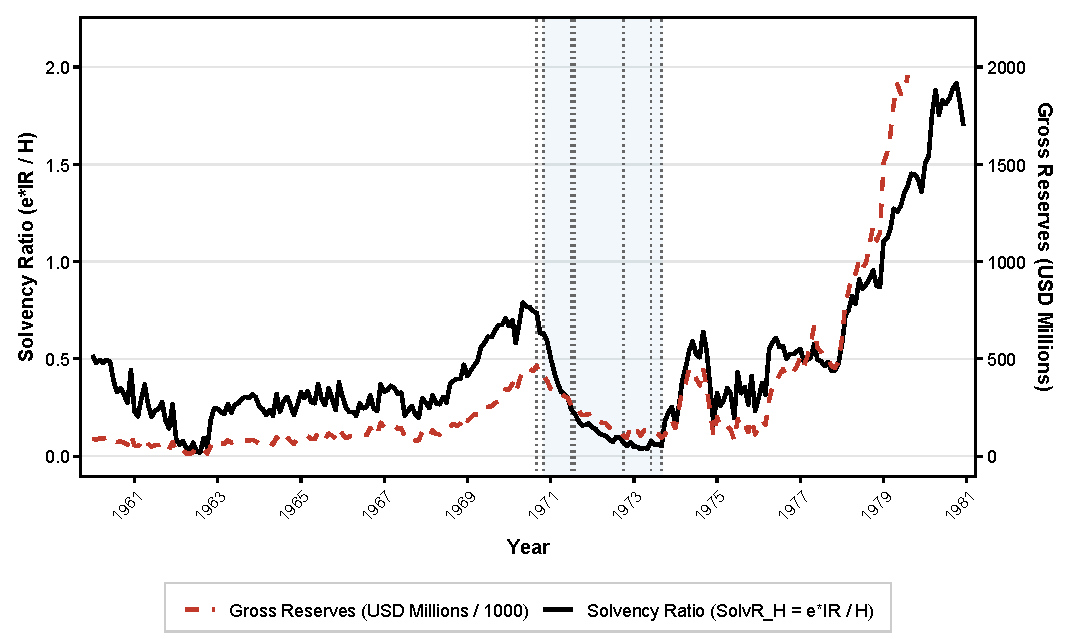
\includegraphics[width=0.88\textwidth]{figures/fig01a_solvency_reserves.pdf}
\begin{minipage}{0.95\textwidth}
\vspace{0.2cm}
\footnotesize
\textbf{Notes:} Monthly series tracking the Central Bank Solvency Ratio relative to Base Money ($\text{SolvR}^{H}_t \equiv \frac{e_t \cdot IR_t}{H_t \cdot 1000}$, left axis, solid black line) and IMF gross international reserves ($IR_t$ in USD millions, right axis, dashed red line). Base money ($H_t$) represents the Central Bank's direct domestic liability base from the archival ledger. Benchmark markers $\mathrm{I}$--$\mathrm{VII}$ defined in Table~\ref{tab:critical_junctures}. Shaded blue region designates the Unidad Popular government (November 1970 -- September 1973). Sourced from Central Bank of Chile REST API and IMF International Financial Statistics.
\end{minipage}
\end{figure}

\begin{figure}[!htbp]
\centering
\caption{World Copper Price and London Gold Price (1960--1980)}
\label{fig:copper_gold}
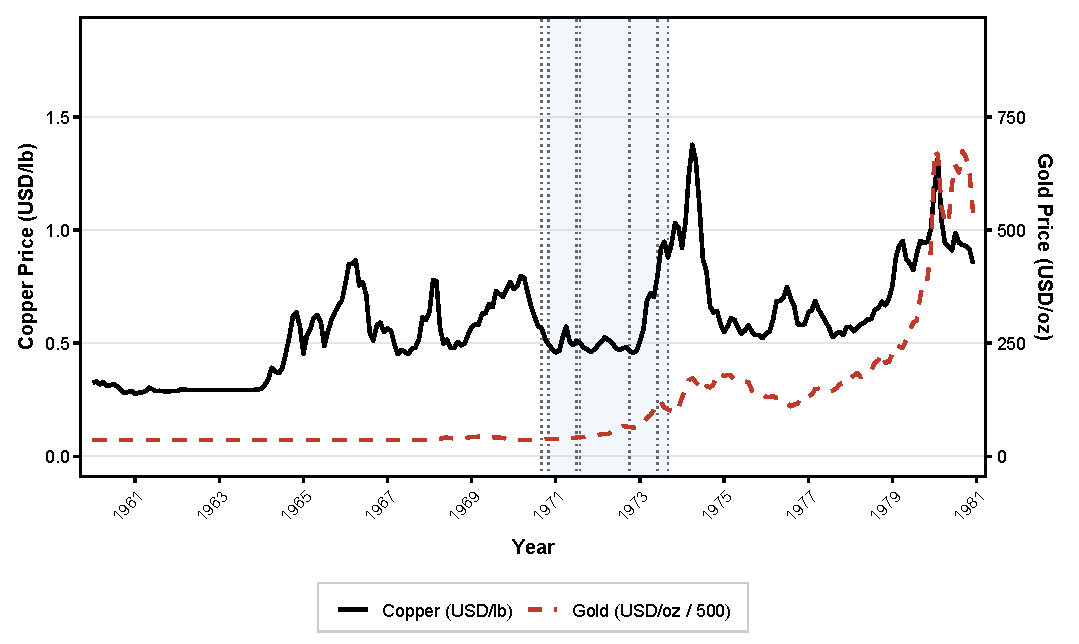
\includegraphics[width=0.88\textwidth]{figures/fig01b_copper_gold.pdf}
\begin{minipage}{0.95\textwidth}
\vspace{0.2cm}
\footnotesize
\textbf{Notes:} Monthly series tracking the London Metal Exchange copper cash price ($P^{\text{Cu}}$ in USD/lb, left axis, solid black line) and London Bullion Market Association gold price ($P^{\text{Gold}}$ in USD/oz / 500, right axis, dashed red line). Benchmark markers $\mathrm{I}$--$\mathrm{VII}$ defined in Table~\ref{tab:critical_junctures}. Shaded blue region designates the Unidad Popular government (November 1970 -- September 1973). Sourced from LME and LBMA via Central Bank of Chile REST API.
\end{minipage}
\end{figure}

The international terms of trade shifted unfavorably during the administration's first year (Figure~\ref{fig:copper_gold}). World copper export prices fell by $25\%$ during 1971, averaging $\$0.47$/lb compared to $\$0.64$/lb across 1969--1970, reducing export revenue during the initial domestic reactivation. Concurrently, the international monetary system absorbed the breakdown of the Bretton Woods architecture following the unilateral suspension of dollar-gold convertibility on August 15, 1971 (Benchmark $\mathrm{IV}$, \citealt{Zoeller2019,Vernengo2021}). The world gold price serves in this chapter as a proxy for the resulting international monetary turbulence and dollar inflation; gold prices rose past $\$100$/oz in 1973 and $\$200$/oz by 1978. In parallel, U.S. wholesale prices rose by $28.0\%$ between late 1970 and mid-1973 (Table~\ref{tab:marglin_monthly_grounding}), raising the foreign-currency price of imported goods.

\begin{figure}[!htbp]
\centering
\caption{Prebisch-ECLAC Real Capacity to Import and Effective Real Imports (1960--1980)}
\label{fig:import_capacity}
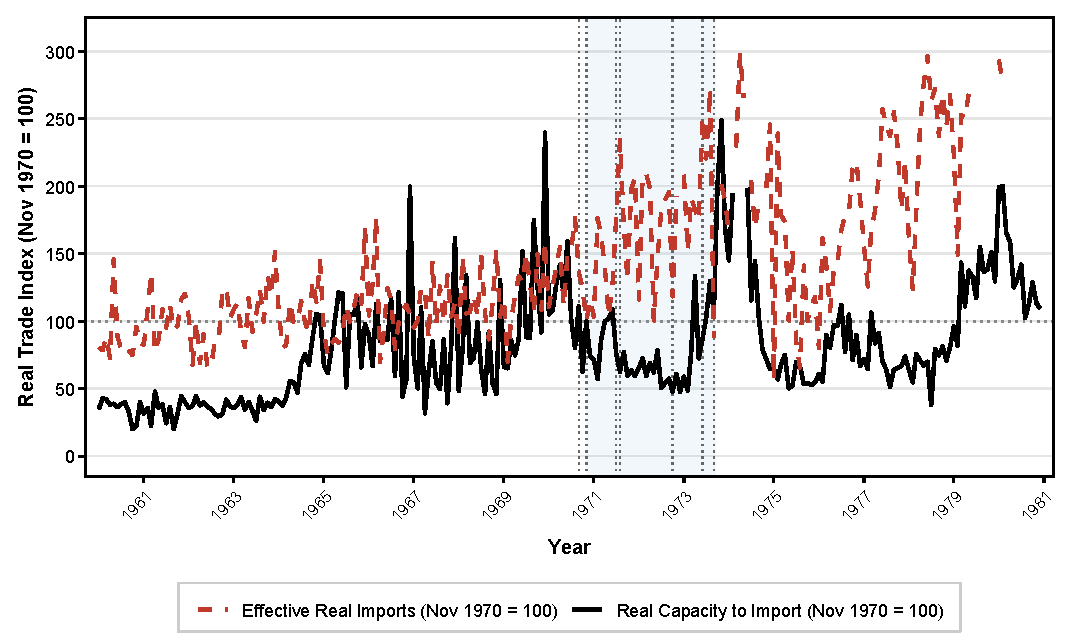
\includegraphics[width=0.88\textwidth]{figures/fig01f_import_capacity.pdf}
\begin{minipage}{0.95\textwidth}
\vspace{0.2cm}
\footnotesize
\textbf{Notes:} Monthly trajectory tracking the Prebisch-ECLAC Real Capacity to Import ($M^{\text{cap}}_t \equiv [\text{Exports}_t / \text{Exports}_{70:11}] \times [(P^{\text{Cu}}_t / P^{\text{Cu}}_{70:11}) / (P^{\text{US}}_{W,t} / P^{\text{US}}_{W,70:11})] \times 100$, solid black line) against Effective Real Imports ($M_t \equiv \text{Imports}_t / \text{Imports}_{70:11} \times 100$, dashed red line). Both series normalized to November 1970 = 100. Benchmark markers $\mathrm{I}$--$\mathrm{VII}$ defined in Table~\ref{tab:critical_junctures}. Shaded blue region designates the Unidad Popular government (1970--1973). Physical merchandise export and import volume series sourced from \citet{DiazBahamonde2023} historical database, compiled from \textit{Estad\'{\i}stica Chilena} and customs records (with April 1973 administrative registration drop interpolated); copper prices from LME via Central Bank of Chile REST API; U.S. wholesale prices from BLS.
\end{minipage}
\end{figure}

Figure~\ref{fig:import_capacity} compares external purchasing power with effective real import flows. When the world price of copper rose from $\$0.508$/lb in January 1973 to $\$0.948$/lb in August 1973, Central Bank gross international reserves remained low, fluctuating in a narrow range of $\$103$--$\$114$ million. The divergence reflected two offsetting movements. On the export side, transport disruptions and equipment shortages held back physical export volumes, muting the revenue gains from higher dollar copper prices. On the import side, effective real imports ($M_t$) expanded, reaching $234.5\%$ of the November 1970 baseline in August 1971 and $272.3\%$ in August 1973, driven by purchases of food, fuel, and intermediate goods.

Operationalizing the Prebisch-ECLAC Capacity to Import ($M^{\text{cap}}_t$), Figure~\ref{fig:import_capacity} documents that Chile's real export purchasing power fell from $100.0$ in November 1970 to $62.5$ in August 1971 and $47.7$ in October 1972 before rebounding in 1973. This generated a wide Real Structural Imbalance ($\Theta_t \equiv M_t / M^{\text{cap}}_t \times 100$), which reached $374.9\%$ in August 1971 and $346.4\%$ in December 1971 (Table~\ref{tab:marglin_monthly_grounding}). The descriptive sequence demonstrates that external balance-of-payments pressures and foreign-exchange scarcity were present well before the price acceleration of late 1972.

\subsubsection{Nominal Dynamics: Money Growth, Inflation, and Multiplier Compression}
\label{sec:stylized_nominal_dynamics}

Figures~\ref{fig:money_growth_inflation} and \ref{fig:money_multiplier} evaluate the high-frequency co-movement between monetary growth, consumer price inflation, and the broad-to-base money multiplier across 1960--1980.

\begin{figure}[!htbp]
\centering
\caption{Monetary Expansion Rates and Monthly Consumer Inflation (1960--1980)}
\label{fig:money_growth_inflation}
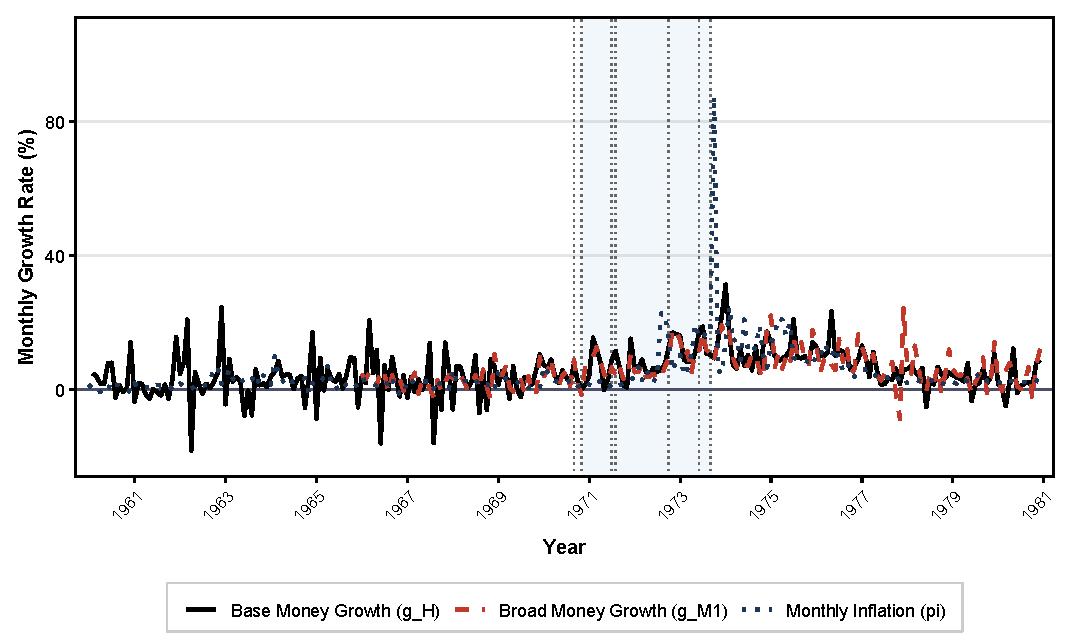
\includegraphics[width=0.88\textwidth]{figures/fig01d_money_growth_inflation.pdf}
\begin{minipage}{0.95\textwidth}
\vspace{0.2cm}
\footnotesize
\textbf{Notes:} Monthly series of base money growth ($g_{H,t}$, solid black line), broad money supply growth ($g_{M1,t}$, dashed red line), and monthly consumer price inflation ($\pi_t$, dotted blue line). Benchmark markers $\mathrm{I}$--$\mathrm{VII}$ defined in Table~\ref{tab:critical_junctures}. Shaded blue region designates the Unidad Popular government (1970--1973). Sourced from Banco Central de Chile REST API and Instituto Nacional de Estad\'{\i}sticas (INE).
\end{minipage}
\end{figure}

\begin{figure}[!htbp]
\centering
\caption{Observed Empirical Money Multiplier ($M1/H$, 1965--1980)}
\label{fig:money_multiplier}
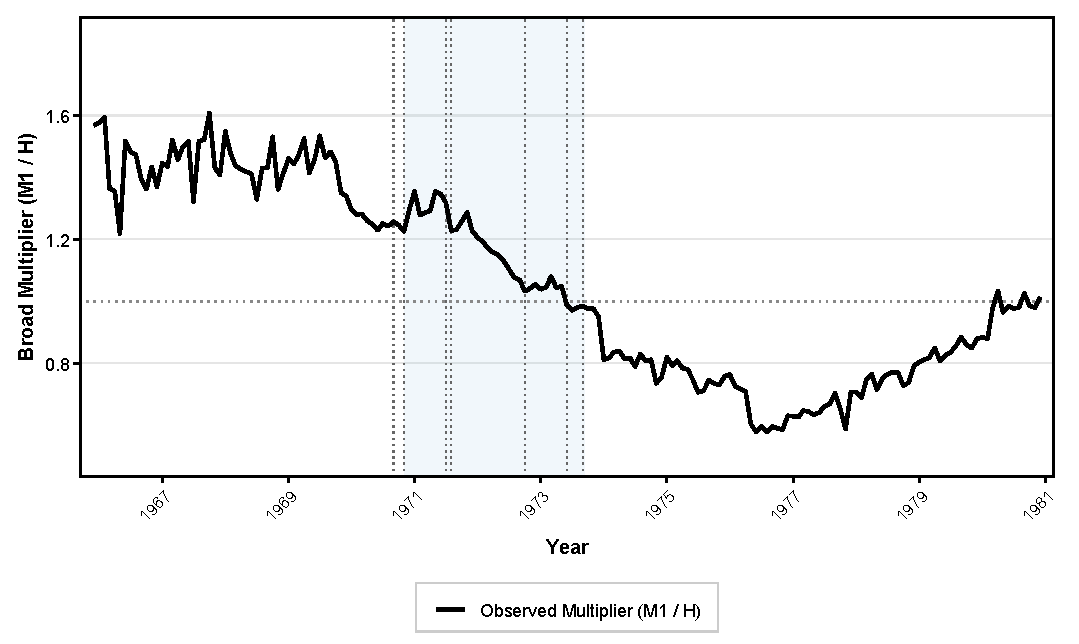
\includegraphics[width=0.88\textwidth]{figures/fig01e_money_multiplier.pdf}
\begin{minipage}{0.95\textwidth}
\vspace{0.2cm}
\footnotesize
\textbf{Notes:} Monthly trajectory of the broad-to-base money multiplier ($m_t \equiv M1_t / H_t$, solid black line). The figure is restricted to the observed M1 sample, December 1965--December 1980. Benchmark markers $\mathrm{I}$--$\mathrm{VII}$ defined in Table~\ref{tab:critical_junctures}. Shaded blue region designates the Unidad Popular government (1970--1973). Sourced from Banco Central de Chile REST API.
\end{minipage}
\end{figure}

In Figure~\ref{fig:money_growth_inflation}, base money ($g_H$) and broad money ($g_{M1}$) grew at monthly rates of $10\%\text{--}15\%$ through 1971 and early 1972, while physical manufacturing output expanded and wages rose. Monthly consumer inflation remained below $5\%$ during this initial phase, rising to $15.2\%$ in October 1972 as transport disruptions and commercial withholding emerged during the nationwide trucking strike. Central bank credit expansion accompanied rising enterprise operating costs and payroll requirements in subsequent months. The monthly peak of consumer inflation occurred in October 1973 ($+87.6\%$) following the military junta's Decree Law 522 price deregulation. This descriptive sequence is consistent with credit accommodation of cost pressures; Section~\ref{sec:granger_tournament} tests whether that directional relationship holds systematically.

Figure~\ref{fig:money_multiplier} tracks the empirical broad-to-base money multiplier ($m_t \equiv M1_t / H_t$). Under Frei (1966--1970), the multiplier fluctuated between $1.35$ and $1.60$. Under the UP administration, the ratio trended downward from $1.35$ in January 1971 to $0.98$ in August 1973, reaching a low of $0.58$ in 1976. Accelerating inflation co-moves visually with this compression in the broad-to-base ratio. Possible institutional mechanisms underlying this decline---including cash hoarding during shortages and central bank credit to socialized firms---are discussed in Sections~\ref{sec:macro_framework} and \ref{sec:discussion_conclusion}; Section~\ref{sec:granger_tournament} evaluates its predictive precedence relative to inflation.

\subsubsection{Real Production Divergence and Focused Monthly Windows}
\label{sec:stylized_real_production}

Figure~\ref{fig:manufacturing_mining} plots physical output dynamics across 1960--1980, documenting divergent paths between domestic manufacturing and export mining.

\begin{figure}[!htbp]
\centering
\caption{Real Physical Output Trajectories: Manufacturing vs. Mining (1960--1980)}
\label{fig:manufacturing_mining}
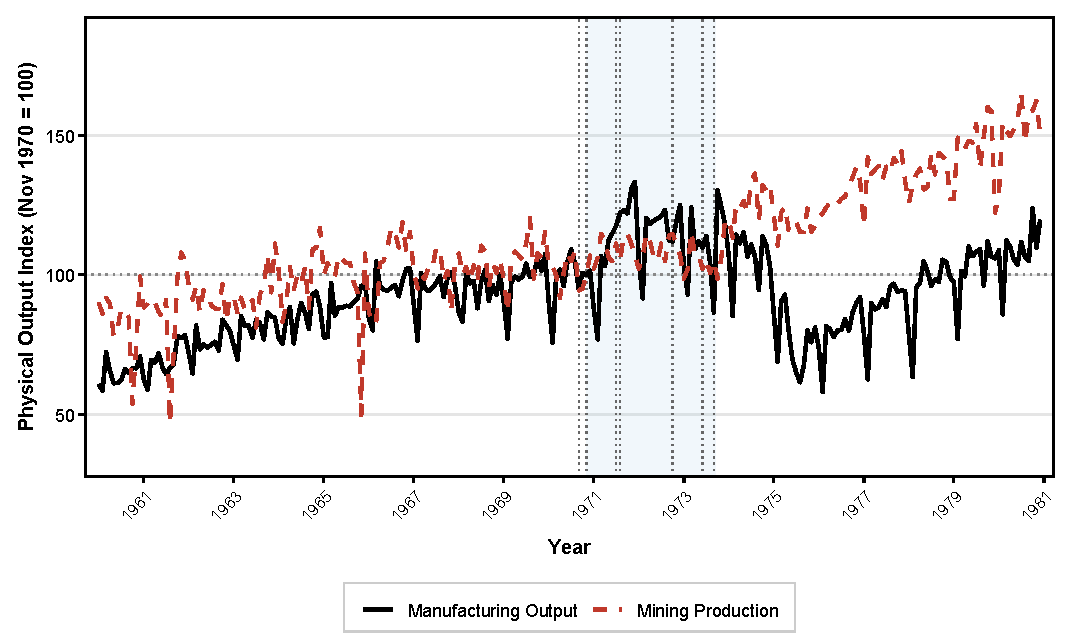
\includegraphics[width=0.88\textwidth]{figures/fig01c_manufacturing_mining.pdf}
\begin{minipage}{0.95\textwidth}
\vspace{0.2cm}
\footnotesize
\textbf{Notes:} Monthly series of physical output indices for manufacturing (solid black line) and mining (dashed red line), re-based to November 1970 = 100. Benchmark markers $\mathrm{I}$--$\mathrm{VII}$ defined in Table~\ref{tab:critical_junctures}. Shaded blue region designates the Unidad Popular government (1970--1973). Sourced from \citet{DiazBahamonde2023} historical database, compiled from INE and SOFOFA for manufacturing, and SERNAGEOMIN, ODEPLAN, and CODELCO for mining.
\end{minipage}
\end{figure}

Manufacturing output expanded by $33.3\%$ between November 1970 and December 1971, reflecting utilization of capacity in wage-goods industries. In contrast, copper mining output rose by $7.0\%$, held back by technical constraints and equipment import delays \citep{DeVylder1976}. Following the October 1972 strike, manufacturing output contracted as transport disruptions and intermediate input shortages took effect. Following the September 1973 coup, manufacturing production declined persistently, falling below index 65 by 1975 (a $>35\%$ contraction from its 1971 peak) amid tariff reductions and demand compression.

Figure~\ref{fig:event_windows} examines monthly dynamics around two institutional turning points.

\begin{figure}[!htbp]
\centering
\begin{subfigure}[b]{0.85\textwidth}
    \centering
    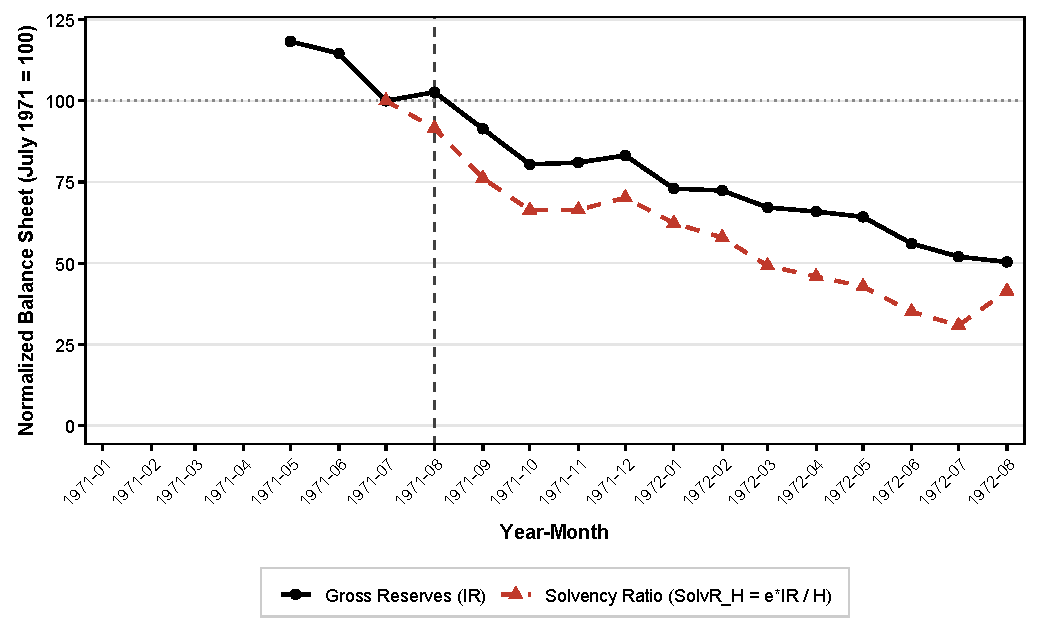
\includegraphics[width=\textwidth]{figures/fig02a_event_blockade_1971.pdf}
    \caption{August 1971 Credit Restrictions and Gold Suspension}
    \label{fig:event_blockade_1971}
\end{subfigure}
\vspace{0.3cm}

\begin{subfigure}[b]{0.85\textwidth}
    \centering
    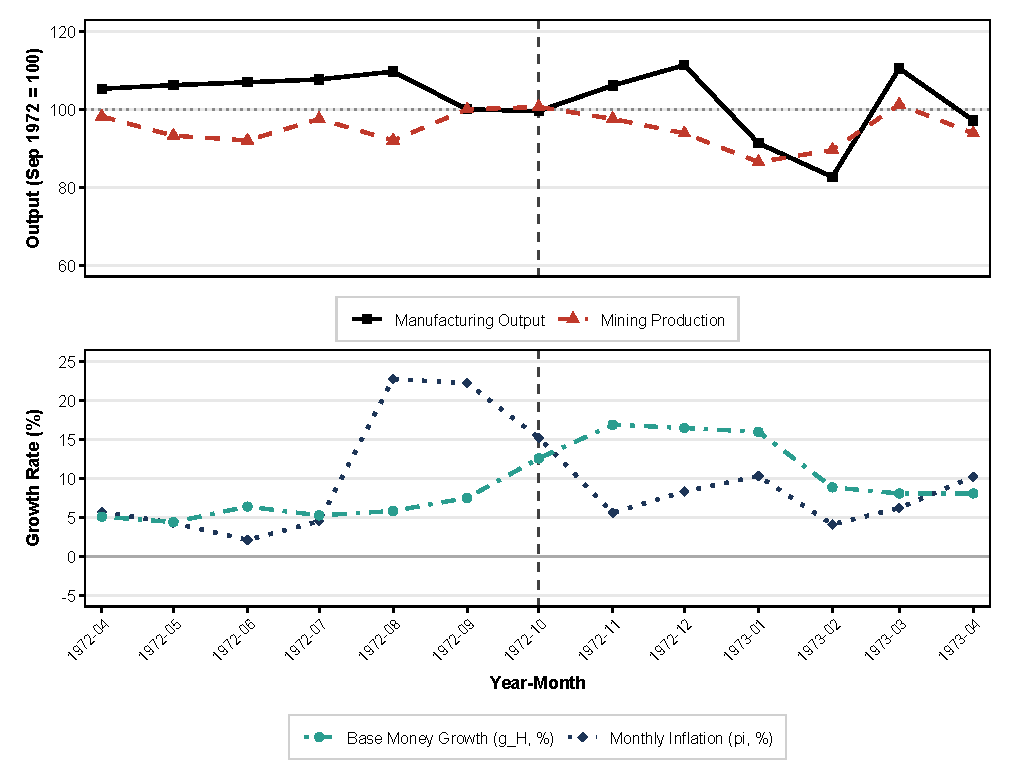
\includegraphics[width=\textwidth]{figures/fig02b_event_lockout_1972.pdf}
    \caption{October 1972 Lockout and Trucking Strike}
    \label{fig:event_lockout_1972}
\end{subfigure}
\caption{Monthly Trajectories around External and Supply Shocks (Chile, 1971--1972)}
\label{fig:event_windows}
\vspace{0.2cm}
\begin{minipage}{0.95\textwidth}
\footnotesize
\textbf{Notes:} Monthly series centered at $t=0$ around two institutional turning points. Panel~(a) tracks Central Bank Gross International Reserves ($IR_t$, solid black line with circle markers) and the Solvency Ratio relative to Base Money ($\text{SolvR}^{H}_t \equiv \frac{e_t \cdot IR_t}{H_t \cdot 1000}$, dashed red line with triangle markers), indexed to July 1971 = 100, around the August 1971 Eximbank credit denial and Bretton Woods gold-window suspension (Benchmark $\mathrm{IV}$). Panel~(b) aligns two vertical subpanels around the October 1972 Lockout (Benchmark $\mathrm{V}$): the upper panel displays physical output indices for Manufacturing (solid black line with square markers) and Mining Production (dashed red line with triangle markers), indexed to September 1972 = 100; the lower panel displays monthly consumer inflation ($\pi_t$, dotted dark-blue line with diamond markers) and Central Bank base money growth ($g_H$, dot-dashed teal line with circle markers) in genuine monthly growth percentages ($\%$) along a common horizontal time axis. Sourced from Banco Central de Chile REST API, IMF International Financial Statistics, and \citet{DiazBahamonde2023}.
\end{minipage}
\end{figure}

The first window centers on the August 1971 credit restrictions and suspension of dollar-gold convertibility (Figure~\ref{fig:event_blockade_1971}, $t=0$). Following the constitutional copper nationalization of July 11, the U.S. Export-Import Bank denied credit on August 12, and President Nixon suspended dollar-gold convertibility on August 15 \citep{Zoeller2019}. This monthly window illustrates the trajectory of reserve drain: gross international reserves fell from index $100.0$ to below $30.0$, and the Central Bank Solvency Ratio ($\text{SolvR}^{H}_t$) declined by more than $70\%$ over the subsequent twelve months. Reserve coverage had deteriorated substantially before the later acceleration in domestic money growth.

The second window centers on the October 1972 trucking strike and commercial lockout (Figure~\ref{fig:event_lockout_1972}, $t=0$). Transport paralysis and merchant shutdowns coincided with a 12 percentage-point drop in manufacturing output, while mining output in northern enclaves remained less affected. Monthly consumer inflation rose from $2.8\%$ to $15.2\%$. Base-money growth did not accelerate contemporaneously with the October jump in inflation; its acceleration followed at $t = +1$ and $t = +2$. The descriptive window places the price increase before the subsequent expansion in base-money growth. While this ordering is consistent with accommodation of cost pressures, establishing directional precedence requires the econometric testing developed below.

\subsubsection{Descriptive Synthesis and Empirical Transition}
\label{sec:stylized_synthesis}

Table~\ref{tab:marglin_monthly_grounding} presents macroeconomic indicators across six selected dates, and Table~\ref{tab:critical_junctures} summarizes the seven institutional events ($\mathrm{I}$--$\mathrm{VII}$).

\begin{table}[H]
\centering
\small
\caption{Monthly Macroeconomic Dynamics, Central Bank Solvency, and External Constraints across Structural Junctures (Chile, 1970--1973)}
\label{tab:marglin_monthly_grounding}
\label{tab:marglin_grounding}
\renewcommand{\arraystretch}{1.10}
\setlength{\tabcolsep}{4.8pt}
\resizebox{\textwidth}{!}{%
\begin{tabular}{lcccccc}
\toprule
& \textbf{Nov 1970} & \textbf{Aug 1971} & \textbf{Dec 1971} & \textbf{Oct 1972} & \textbf{Aug 1973} & \textbf{Dec 1973} \\
\textbf{Macroeconomic Variable} & \textit{Inauguration} & \textit{Gold Suspension} & \textit{Output Peak} & \textit{October Lockout} & \textit{Pre-Coup} & \textit{Post-Coup} \\
\midrule
\multicolumn{7}{l}{\textbf{A. Inflation and Price Dynamics}} \\[0.2em]
Monthly Inflation (\%) & 0.6\% & 1.1\% & 2.8\% & 15.2\% & 17.1\% & 4.7\% \\
YoY Inflation (\%) & 35.3\% & 17.4\% & 22.1\% & 142.9\% & 303.6\% & 508.1\% \\
\midrule
\multicolumn{7}{l}{\textbf{B. Real Physical Activity (Nov 1970 = 100)}} \\[0.2em]
Manufacturing Output Index & 100.0 & 122.0 & 133.3 & 111.9 & 104.6 & 118.1 \\
Mining Production Index & 100.0 & 104.9 & 107.0 & 114.7 & 100.7 & 119.6 \\
\midrule
\multicolumn{7}{l}{\textbf{C. Central Bank Solvency and Monetary Backing}} \\[0.2em]
Gross International Reserves (USD M) & 408.0 & 268.1 & 217.2 & 103.4 & 114.2 & 179.7 \\
Solvency Ratio Base ($\text{SolvR}^H \equiv \frac{e \cdot IR}{H \cdot 1000}$) & 0.63 & 0.22 & 0.17 & 0.07 & 0.06 & 0.25 \\
Solvency Ratio M1 ($\text{SolvR}^{M1} \equiv \frac{e \cdot IR}{M1 \cdot 1000}$) & 0.51 & 0.18 & 0.14 & 0.07 & 0.06 & 0.27 \\
Observed Multiplier ($M1/H$) & 1.23 & 1.23 & 1.23 & 1.03 & 0.98 & 0.95 \\
Base Money Monthly Growth ($g_H$) & 0.0\% & 11.5\% & 15.1\% & 12.6\% & 10.7\% & 21.8\% \\
M1 Money Monthly Growth ($g_{M1}$) & -1.6\% & 4.3\% & 10.2\% & 9.1\% & 11.6\% & 19.2\% \\
\midrule
\multicolumn{7}{l}{\textbf{D. Official Exchange Rate and World Commodity Prices}} \\[0.2em]
Official Exchange Rate ($e_t$) & 0.012 & 0.0122 & 0.0146 & 0.0250 & 0.0740 & 0.34 \\
World Copper Price (USD/lb) & \$0.492 & \$0.499 & \$0.471 & \$0.466 & \$0.948 & \$1.011 \\
World Gold Price (USD/oz) & \$37.44 & \$42.71 & \$43.48 & \$64.86 & \$106.76 & \$106.72 \\
\midrule
\multicolumn{7}{l}{\textbf{E. External Trade, Capacity to Import, and Structural Imbalance}} \\[0.2em]
Export Activity Index & 2.68 & 1.71 & 1.73 & 1.46 & 2.31 & 2.81 \\
Import Activity Index & 1.51 & 3.54 & 3.11 & 1.79 & 4.11 & 2.86 \\
Real Trade Ratio ($\text{Exp}/\text{Imp}$) & 1.78 & 0.48 & 0.56 & 0.82 & 0.56 & 0.98 \\
Real Capacity to Import ($M^{\text{cap}}_t$, Nov 1970 = 100) & 100.0 & 62.5 & 59.5 & 47.7 & 129.5 & 168.7 \\
Effective Real Imports ($M_t$, Nov 1970 = 100) & 100.0 & 234.5 & 206.2 & 118.4 & 272.3 & 189.4 \\
Real Structural Imbalance ($\Theta_t$, \%) & 100.0\% & 374.9\% & 346.4\% & 248.1\% & 210.3\% & 112.3\% \\
US Wholesale Price Index (Nov 1970 = 100) & 100.0 & 103.8 & 104.0 & 108.1 & 128.0 & 127.8 \\
\bottomrule
\end{tabular}%
}
\vspace{0.3em}
\begin{minipage}{\textwidth}
\footnotesize \textbf{Sources and Notes:} Primary monthly series from Central Bank of Chile and IMF International Financial Statistics. Gross international reserves ($IR_t$) represent official foreign exchange holdings from IMF IFS. Solvency Ratio defined relative to Base Money as $\text{SolvR}^{H}_t \equiv (e_t \cdot IR_t) / (H_t \cdot 1000)$ and relative to M1 as $\text{SolvR}^{M1}_t \equiv (e_t \cdot IR_t) / (M1_t \cdot 1000)$, where $IR_t$ is in USD millions, $e_t$ is the official exchange rate in pesos per USD (standardized per BCCh historical conventions), and $H_t, M1_t$ are recorded in thousands of millions of pesos (billions, \emph{miles de millones de pesos}), scaled by $1{,}000$ to express monetary liabilities in millions of pesos and ensure dimensional consistency with the numerator ($e_t \cdot IR_t$). Capacity to Import Index operationalizes the Prebisch-ECLAC formula: $M^{\text{cap}}_t \equiv (\text{Exports}_t / \text{Exports}_{70:11}) \times [(P^{\text{Cu}}_t / P^{\text{Cu}}_{70:11}) / (P^{\text{US}}_{W,t} / P^{\text{US}}_{W,70:11})] \times 100$. Real Structural Imbalance Ratio defined as $\Theta_t \equiv (M_t / M^{\text{cap}}_t) \times 100$, tracking the physical quantum of imports relative to real export purchasing power. Selected dates mark historical milestones: Nov 1970 (Allende inauguration baseline); Aug 1971 (Eximbank credit denial and suspension of dollar-gold convertibility); Dec 1971 (cyclical output peak); Oct 1972 (national trucking strike and commercial lockout); Aug 1973 (late administration baseline before the September coup); and Dec 1973 (post-coup benchmark following October 1973 Decree Law 522 price deregulation).
\end{minipage}
\end{table}


\begin{table}[H]
\centering
\small
\caption{Chronology of Critical Macroeconomic Junctures and Institutional Shocks (Chile, 1970--1973)}
\label{tab:critical_junctures}
\renewcommand{\arraystretch}{1.15}
\resizebox{\textwidth}{!}{%
\begin{tabular}{clllp{6.8cm}}
\toprule
\textbf{Ref} & \textbf{Date} & \textbf{Historical Juncture} & \textbf{Institutional Shock Mechanism} & \textbf{Macroeconomic / Balance-Sheet Transmission Channel} \\
\midrule
$\mathrm{I}$   & Sep 1970 & Presidential Election & Electoral panic; commercial deposit runs & Capital flight ($EO < 0$); foreign currency accumulation; Central Bank emergency rediscounts. \\
$\mathrm{II}$  & Nov 1970 & Inauguration Baseline & Allende assumes presidency; tariff and price freeze & Initial price stabilization; real wage gains; inherited gross reserve buffer (\$408.0M; $\text{SolvR}^H = 0.63$; $\text{SolvR}^{M1} = 0.51$). \\
$\mathrm{III}$ & Jul 1971 & Copper Nationalization & Unanimous constitutional reform (Law 17,450) & Sovereign recovery of \textit{Gran Miner\'ia}; triggers bilateral U.S. credit restrictions and legal liens. \\
$\mathrm{IV}$  & Aug 1971 & Eximbank Embargo \& Bretton Woods Collapse & U.S. credit freeze; dollar-gold convertibility suspended & Revolving trade credits reduced (\$220M $\to$ \$35M); cash-in-advance imports; reserve drain accelerates ($\Delta IR = -\$140$M). \\
$\mathrm{V}$   & Oct 1972 & October Lockout (\textit{Paro de Octubre}) & Trucking strike; SOFOFA commercial lockout & Physical transport paralysis; wholesale inventory withholding; monthly inflation rises to $15.2\%$; central bank liquidity accommodation. \\
$\mathrm{VI}$  & Jun 1973 & \textit{El Tanquetazo} & Military uprising (2nd Armored Regiment) & Heightened political instability; logistical disruption; black market expansion; reserve depletion and structural trade imbalance ($\Theta_t = 210.3\%$). \\
$\mathrm{VII}$ & Sep 1973 & Military Coup d'\'Etat & Violent overthrow; followed by October DL 522 deregulation & Elimination of price controls; $+87.6\%$ MoM inflation jump in October; real wage contraction ($-40\%$); domestic expenditure compression. \\
\bottomrule
\end{tabular}%
}
\begin{tabular}{p{0.95\textwidth}}
\footnotesize \textbf{Notes:} Master reference chronology for vertical benchmark lines appearing across high-frequency time series (Figures~\ref{fig:solvency_reserves}--\ref{fig:money_multiplier}) and defining intervention cutoffs for focused monthly windows (Figures~\ref{fig:event_blockade_1971}--\ref{fig:event_lockout_1972}) and companion econometric estimation stages.
\end{tabular}
\end{table}


Table~\ref{tab:marglin_monthly_grounding} illustrates this temporal sequence across the selected dates: between November 1970 and August 1971---while monthly consumer inflation remained low ($1.1\%$) and industrial manufacturing output was expanding ($+22.0\%$)---the Central Bank Solvency Ratio ($\text{SolvR}^{H}_t$) had declined from $0.63$ to $0.22$, and gross foreign reserves had fallen by $\$139.9$ million. External balance-of-payments deterioration preceded the subsequent acceleration of domestic inflation and credit expansion.

Across the selected dates, reserve coverage deteriorated substantially before the sharp acceleration of inflation in late 1972. Money growth, inflation, exchange-rate adjustment, and trade imbalances moved together during much of the crisis, so these descriptive sequences do not establish their direction of dependence. Section~\ref{sec:granger_tournament} evaluates directional predictive precedence through Granger-causality tests in stationary vector autoregressions across six modular empirical systems. Section~\ref{sec:tvar_solvency_regimes} then estimates a non-linear Threshold Vector Autoregression (TVAR) conditioned on the monthly Solvency Growth Gap ($\Delta s_{t-1} \equiv g^F_{t-1} - g^H_{t-1}$) to test whether these relationships change under conditions of central bank insolvency.



\subsection{Empirical Exercise 1: Directional Precedence and Monetary Accommodation in Stationary Vector Autoregressions}
\label{sec:granger_tournament}
\label{sec:granger_linear}

\subsubsection{Econometric Framework and Evidential Standard}
\label{sec:granger_methodology}
\label{sec:granger_unit_root}
\label{sec:granger_tournament_setup}

The stylized facts documented in Section~\ref{sec:stylized_facts} leave open a central empirical question: did domestic monetary expansion precede price acceleration as an autonomous impulse, or did it accommodate price pressures, enterprise working-capital requirements, and external balance-of-payments constraints? Standard monetarist accounts treat money creation as an autonomous driver, implying that high-powered reserve money ($g_{H,t}$) and narrow transactions balances ($g_{M1,t}$) should expand without predictive feedback from consumer prices ($\pi_t$) or external shocks:
\begin{equation}
    \mathcal{H}_0^{\text{Exogenous}}: \quad \pi_{t-k} \not\longrightarrow g_{M,t} \quad \text{and} \quad \text{External Shock}_{t-k} \not\longrightarrow g_{M,t} \quad \forall k \ge 1.
    \label{eq:null_exogeneity}
\end{equation}
In contrast, structuralist and endogenous-money frameworks view money creation as an accommodating response to enterprise cost pressures and balance-of-payments disruptions. When enterprises face escalating nominal costs under price controls and supply bottlenecks, working-capital requirements expand. If the monetary authority accommodates these demands to prevent illiquidity and payroll defaults, temporal predictive precedence should flow from inflation and foreign reserve depletion to domestic money growth ($\pi \to g_H$, $\text{SolvR}^H \to g_H$).

To evaluate these competing temporal sequences, I estimate standard Granger-causality tests within stationary vector autoregressions \citep{Hamilton1994,Lutkepohl2005}. Let $Y_t$ denote a $K \times 1$ vector of stationary transformed macroeconomic series ($I(0)$). An unrestricted vector autoregression of order $k$, $\text{VAR}(k)$, is specified:
\begin{equation}
    Y_t = c + \sum_{i=1}^k A_i Y_{t-i} + \varepsilon_t, \label{eq:var_spec}
\end{equation}
where $c$ is a vector of constants, $A_i$ are $K \times K$ coefficient matrices, and $\varepsilon_t$ is a vector of white-noise disturbances. In a bivariate representation for $(y_t, x_t)$, the system reduces to:
\begin{align}
    y_t &= \alpha_0 + \sum_{i=1}^k \alpha_{i} y_{t-i} + \sum_{i=1}^k \delta_{i} x_{t-i} + \varepsilon_{1t}, \label{eq:granger_spec1} \\
    x_t &= \beta_0 + \sum_{i=1}^k \beta_{i} x_{t-i} + \sum_{i=1}^k \phi_{i} y_{t-i} + \varepsilon_{2t}. \label{eq:granger_spec2}
\end{align}
The null hypothesis that $x_t$ does not Granger-cause $y_t$ corresponds to the joint exclusion restriction on the lagged coefficients of $x$:
\begin{equation}
    H_0: \quad \delta_{1} = \dots = \delta_{k} = 0.
\end{equation}
Because the entered series are stationary ($I(0)$, as established by the Augmented Dickey--Fuller tests in Table~\ref{tab:adf_order_integration}), this restriction is tested using standard finite-sample $F$-tests:
\begin{equation}
    F = \frac{(\text{RSS}_R - \text{RSS}_U) / k}{\text{RSS}_U / (T - Kk - 1)} \sim F(k, T - Kk - 1),
\end{equation}
where $\text{RSS}_R$ and $\text{RSS}_U$ denote the residual sums of squares from the restricted and unrestricted models, respectively. Rejecting $H_0$ indicates that lagged values of $x_t$ contain incremental predictive information for $y_t$ beyond what is captured by the remaining lagged variables in the system. 

In accordance with the chapter's causal-language contract, Granger causality denotes incremental predictive precedence within a specified stationary information set; it does not by itself establish structural causal identification or policy invariance. Empirical admission to the main text is governed by three diagnostic criteria: (1)~modulus stability ($\max |\lambda_i| < 1$); (2)~system-level residual whitening via the multivariate Breusch--Godfrey Lagrange Multiplier test ($p > 0.05$); and (3)~equation-level residual whitening ($p > 0.05$). Specifications that fail these diagnostic standards are not used for directional inference in the main text.

Table~\ref{tab:system_definitions} defines the system variable vectors, mathematical transformations, sample coverage, and evidence status across the empirical systems.
\begin{table}[htbp]
\centering
\small
\renewcommand{\arraystretch}{0.88}
\caption{System Variable Specification and Evidence Hierarchy}
\label{tab:system_definitions}
\begin{tabularx}{\textwidth}{llcc>{\RaggedRight}X}
\toprule
\textbf{System} & \textbf{Variable Vector $Y^{(s)}_t$} & \textbf{$K$} & \textbf{Evidence Status} & \textbf{Variable Definitions and Historical Sample} \\
\midrule
\multicolumn{5}{l}{\textbf{Core Empirical Specifications (Main Text)}} \\
\midrule
\textbf{System 1} & $[\pi_t, \; g_{H,t}]'$ & 2 & Robust Linear & $\pi_t$: Monthly CPI inflation ($\Delta \ln \text{CPI}_t \times 100$). \newline $g_{H,t}$: Base money growth ($\Delta \ln H_t \times 100$). \newline Sample: 1960:01--1980:12 ($N=250$, usable $N_{\text{eff}}=247$). \\
\addlinespace[0.3em]
\textbf{System 2} & $[\pi_t, \; g_{M1,t}, \; g_{H,t}]'$ & 3 & Qualified Linear & $\pi_t$: CPI inflation. \newline $g_{M1,t}$: Un-spliced narrow money growth ($\Delta \ln M1_t \times 100$). \newline $g_{H,t}$: Base money growth. \newline Sample: 1966:01--1980:12 ($N=180$, usable $N_{\text{eff}}=177$). \\
\addlinespace[0.3em]
\textbf{System 6} & $[g_{\text{SolvR\_H},t}, \; g_{P,\text{gold},t}, \; g_{e,t}, \; g_{H,t}, \; \pi_t]'$ & 5 & Qualified Linear (Pre-73) & $g_{\text{SolvR\_H},t}$: Central bank solvency ratio growth ($\text{SolvR}_t^H \equiv [e_t \cdot \text{IR}_t] / [H_t \cdot 1000]$). \newline $g_{P,\text{gold},t}$: World gold price growth. \newline $g_{e,t}$: Devaluation rate. \newline $g_{H,t}$: Base money growth; $\pi_t$: CPI inflation. \newline Sample: 1960:02--1973:09 ($N_{\text{eff}}=161$). \\
\midrule
\multicolumn{5}{l}{\textbf{Auxiliary and Sensitivity Specifications}} \\
\midrule
\textbf{System 3} & $[\pi_t, \; g_{H,t}, \; \Delta \ln m_t]'$ & 3 & Sensitivity Note & $\Delta \ln m_t$: Banking multiplier growth ($m_t \equiv M1_t / H_t$). Sensitivity check on banking mechanism (1966--1980, $N=180$). \\
\addlinespace[0.3em]
\textbf{System 4} & $[\pi_t, \; g_{H,t}, \; \Delta \ln \Theta_t, \; g_{\text{Manuf},t}, \; g_{\text{Mining},t}]'$ & 5 & Descriptive Only & $\Delta \ln \Theta_t$: Structural import imbalance growth; $g_{\text{Manuf},t}$: Manufacturing; $g_{\text{Mining},t}$: Mining. Retained in Appendix~\ref{app:linear_var_diagnostics}. \\
\addlinespace[0.3em]
\textbf{System 5} & $[g_{P,\text{gold},t}, \; g_{e,t}, \; \Delta \ln \Theta_t, \; g_{H,t}, \; \pi_t]'$ & 5 & Inconclusive & External cost-push boundary vector. Unresolved residual autocorrelation; retained in Appendix~\ref{app:linear_var_diagnostics}. \\
\bottomrule
\end{tabularx}
\begin{minipage}{\textwidth}
\vspace{0.3em}
\footnotesize \textit{Notes:} Monthly series from the Central Bank of Chile (BCCh) historical databases and IMF International Financial Statistics. All variables enter in stationary form ($I(0)$). Classification reflects the empirical architecture lock: Systems 1, 2, and qualified pre-October 1973 System 6 constitute the admissible linear core; System 3 is a sensitivity check; Systems 4 and 5 are documented in Appendix~\ref{app:linear_var_diagnostics}.
\end{minipage}
\end{table}


\subsubsection{Nominal Accommodation: Money and Inflation}
\label{sec:granger_nominal_core}

System 1 evaluates dynamic feedback between consumer price inflation ($\pi_t$) and high-powered base money growth ($g_{H,t}$) over the full monthly sample (1960:01--1980:12, $N=250$, usable $N_{\text{eff}}=247$ at lag 4). At lag order $k=4$, the system satisfies all diagnostic admissibility criteria: companion matrix eigenvalues confirm stability ($\max |\lambda| = 0.730$), the system Breusch--Godfrey test indicates an absence of residual autocorrelation ($\chi^2 = 3.06, p = 0.548$), and equation-level Breusch--Godfrey tests confirm whitening in both the base money equation ($p = 0.467$) and the inflation equation ($p = 0.284$).

As reported in Panel~A of Table~\ref{tab:core_granger_evidence}, Granger causality between inflation and base money growth is bidirectional at $k=4$. The null that inflation does not Granger-cause base money growth is rejected at the 0.1\% level ($F = 15.004, p < 0.0001$), with a positive sum of lag coefficients ($\sum \hat{\beta}_i = +0.680$). In the forward direction, base money growth also Granger-causes inflation ($F = 2.718, p = 0.0305, \sum \hat{\beta}_i = +0.380$). Evaluating results across alternative lag lengths confirms that reverse accommodation ($\pi \to g_H$) commands substantially larger test statistics ($F \in [15.00, 28.32], p < 0.0001$ across $k=1,\dots,4$) and maintains unbroken statistical significance at all horizons. Forward money growth ($g_H \to \pi$) predicts inflation strongly at short horizons ($F = 14.557, p = 0.0002$ at $k=1$; $F = 9.284, p = 0.0001$ at $k=2$), but attenuates as lag length increases (at the SBIC-selected lag $k^*=3$, $\pi \to g_H$ yields $F = 20.318, p < 0.0001$ while $g_H \to \pi$ yields $F = 5.544, p = 0.0011$).

This pattern provides evidence consistent with defensive monetary accommodation under acute price pressures. While high-powered money growth contributed to subsequent price acceleration at short horizons, consumer price inflation exerted strong and persistent predictive feedback on base money creation. The bidirectional finding is difficult to reconcile with the strict monetarist premise of unidirectional money exogeneity, while demonstrating that nominal transmission operated as a reciprocal spiral. System 1 is classified as a \textsc{Robust Linear Result}.

\subsubsection{Commercial Banking and Multiplier Sensitivity}
\label{sec:granger_banking}

System 2 evaluates the commercial banking sector using official un-spliced narrow money balances ($M1$), high-powered base money ($H$), and consumer price inflation over the post-1966 banking window (1966:01--1980:12, $N=180$, usable $N_{\text{eff}}=177$ at $k=3$). At lag $k=3$, the three-variable system satisfies the diagnostic admissibility criteria: the system is stable ($\max |\lambda| = 0.817$), the system Breusch--Godfrey test fails to reject white-noise residuals ($p = 0.428$), and equation-level tests indicate no serial correlation ($p = 0.289$ in the base money equation).

As shown in Panel~B of Table~\ref{tab:core_granger_evidence}, in the diagnostically admissible trivariate VAR(3), narrow-money and base-money growth contain predictive information for one another after conditioning on inflation. Commercial narrow-money growth predicts base-money expansion ($g_{M1} \to g_H$: $F = 3.654, p = 0.0138, \sum \hat{\beta}_i = +0.510$), while base-money growth also predicts narrow money ($g_H \to g_{M1}$: $F = 3.239, p = 0.0236, \sum \hat{\beta}_i = +0.333$). Inflation also predicts subsequent narrow-money growth ($\pi \to g_{M1}$: $F = 6.842, p = 0.0002, \sum \hat{\beta}_i = +0.284$). The reverse relation is not detected once base-money growth is included in the information set: the null that narrow-money growth does not Granger-cause inflation cannot be rejected ($g_{M1} \to \pi$: $F = 1.004, p = 0.3927, \sum \hat{\beta}_i = +0.444$). The banking specification therefore supports predictive interaction between narrow and base money, while the pairwise relation from narrow-money growth to inflation does not survive conditioning on the monetary base. This bilateral dynamic is consistent with an endogenous reserve response to commercial-bank transactions balances, though predictive relations between broad monetary aggregates do not structurally identify credit supply from credit demand. System 2 is classified as a \textsc{Qualified Linear Result}.

\paragraph{Sensitivity Note: Money Multiplier Deconstruction (System 3).}
Deconstructing narrow money into base money and the banking multiplier ($m_t \equiv M1_t / H_t$) evaluates whether multiplier expansion autonomously preceded inflation. In bivariate pairwise tests ($k=1$), multiplier growth displays no predictive information for price inflation ($F = 0.338, p = 0.5617$). When estimated within a conditional VAR(1) containing base money growth, the predictive link $\Delta \ln m \to \pi$ shifts to marginal statistical significance ($F = 3.896, p = 0.0484$). The multiplier result is sensitive to the conditioning set. Because multiplier growth is algebraically related to narrow-money and base-money growth ($\Delta \ln m_t \equiv g_{M1,t} - g_{H,t}$), conditioning on base money growth mathematically incorporates narrow money dynamics, closely reflecting the commercial credit interaction documented in System~2. This specification is therefore treated as a sensitivity check on the banking representation rather than as an independent empirical result, and is classified as \textsc{Specification-Sensitive}.

\subsubsection{Central Bank Solvency Dynamics Before October 1973}
\label{sec:granger_solvency_pre73}

System 6 examines the dynamic interaction between the central bank's foreign solvency backing and domestic macroeconomic aggregates. The system specifies the five-variable vector $Y^{(6)}_t = [g_{\text{SolvR\_H},t}, g_{P,\text{gold},t}, g_{e,t}, g_{H,t}, \pi_t]'$, where $g_{\text{SolvR\_H},t} \equiv \Delta \ln \text{SolvR}^H_t \times 100$ tracks the monthly growth rate of the Solvency Ratio ($\text{SolvR}^H_t \equiv [e_t \cdot \text{IR}_t] / [H_t \cdot 1000]$).

In the full sample (1960:01--1980:12, $N=250$), System 6 fails residual whitening across all tested lag lengths $k \in \{1, \dots, 4\}$ ($p < 0.0001$). Under the chapter's admissibility criteria, the full-sample linear system is not used for directional inference. However, partitioning the sample at the October 1973 institutional break reveals that residual autocorrelation is concentrated in the post-1973 crawling-peg era. In the pre-October 1973 subperiod (1960:02--1973:09, $N_{\text{eff}} = 161$), extending the specification to $k=3$ resolves residual persistence. The pre-1973 conditional VAR(3) is the unique specification across all tested sample partitions that satisfies all serial-admissibility criteria: the companion matrix is stable ($\max |\lambda| = 0.8817$), the system Breusch--Godfrey test indicates white-noise residuals ($\chi^2 = 116.35, df=100, p = 0.1262$), the minimum equation-level Breusch--Godfrey test is satisfied ($p = 0.0557$ in the base money equation), and the 12-month Portmanteau test confirms absence of residual correlation ($p = 0.0754$).

Panel~C of Table~\ref{tab:core_granger_evidence} reports the conditional Granger causality results for this admissible pre-1973 model. Solvency ratio growth predictively Granger-causes base money growth ($F = 6.983, p = 0.0002$), driven by a statistically significant positive coefficient at lag 3 ($\hat{\beta}_3 = +0.0568, p = 0.0033$; sum $\sum \hat{\beta}_i = +0.0153$). In the reverse direction, base money growth predictively Granger-causes solvency ratio growth ($F = 2.951, p = 0.0347$), with a large negative coefficient concentrated at lag 2 ($\hat{\beta}_2 = -0.9775, p = 0.0074$; sum $\sum \hat{\beta}_i = -0.8365$). Because high-powered money enters directly into the denominator of $\text{SolvR}^H_t$, this negative predictive lag is consistent with subsequent deterioration in reserve backing, partly reflecting the mechanical denominator relation rather than offsetting reserve accumulation. Solvency ratio growth also contains predictive information for nominal exchange-rate adjustments ($g_{\text{SolvR\_H}} \to g_e$: $F = 3.073, p = 0.0297, \sum \hat{\beta}_i = +0.129$). Consumer price inflation does not predict solvency growth in this conditional specification ($F = 0.686, p = 0.5618$).

These findings establish a qualified empirical result: prior to October 1973, domestic base money creation predicts a decline in the central bank's foreign solvency ratio (partly reflecting the denominator relation), while foreign solvency dynamics exerted lagged predictive feedback on monetary emission. Because this relationship cleared diagnostic standards only within the pre-October 1973 subperiod and cannot be established as a time-invariant linear law across the full sample, System 6 is classified as a \textsc{Qualified Linear Result (Pre-October 1973 Only)}. The linear specification does not determine whether these predictive relationships vary with the inherited solvency state. Section~\ref{sec:tvar_solvency_regimes} examines that possibility directly.

\begin{table}[htbp]
\centering
\small
\renewcommand{\arraystretch}{0.92}
\caption{Admissible Linear Granger Directional Precedence and Evidence Hierarchy}
\label{tab:core_granger_evidence}
\resizebox{\textwidth}{!}{%
\begin{tabular}{llcccccc}
\toprule
\textbf{Direction Tested} & \textbf{Information Set / Regressors} & \textbf{Lag ($k$)} & \textbf{$F$-Statistic} & \textbf{$p$-value} & \textbf{$\sum \hat{\beta}_i$} & \textbf{Diagnostic Status} & \textbf{Evidence Hierarchy} \\
\midrule
\multicolumn{8}{l}{\textbf{Panel A: System 1 --- Nominal Core (Full Sample, 1960:01--1980:12, $N=250$, $N_{\text{eff}}=247$)}} \\
\midrule
$\pi_t \longrightarrow g_{H,t}$ & $\{\pi_t, g_{H,t}\}$ & 4 & 15.004$^{***}$ & $< 0.0001$ & $+0.680$ & Pass (Sys BG $p=0.548$; Eq $p=0.467$) & \textsc{Robust Linear Result} \\
$g_{H,t} \longrightarrow \pi_t$ & $\{\pi_t, g_{H,t}\}$ & 4 & 2.718$^{**}$ & 0.0305 & $+0.380$ & Pass (Sys BG $p=0.548$; Eq $p=0.467$) & \textsc{Robust Linear Result} \\
\midrule
\multicolumn{8}{l}{\textbf{Panel B: System 2 --- Commercial Banking (M1 Window, 1966:01--1980:12, $N=180$, $N_{\text{eff}}=177$)}} \\
\midrule
$g_{M1,t} \longrightarrow g_{H,t}$ & $\{\pi_t, g_{M1,t}, g_{H,t}\}$ & 3 & 3.654$^{**}$ & 0.0138 & $+0.510$ & Pass (Sys BG $p=0.428$; Eq $p=0.289$) & \textsc{Qualified Linear Result} \\
$g_{H,t} \longrightarrow g_{M1,t}$ & $\{\pi_t, g_{M1,t}, g_{H,t}\}$ & 3 & 3.239$^{**}$ & 0.0236 & $+0.333$ & Pass (Sys BG $p=0.428$; Eq $p=0.289$) & \textsc{Qualified Linear Result} \\
$\pi_t \longrightarrow g_{M1,t}$ & $\{\pi_t, g_{M1,t}, g_{H,t}\}$ & 3 & 6.842$^{***}$ & 0.0002 & $+0.284$ & Pass (Sys BG $p=0.428$; Eq $p=0.289$) & \textsc{Qualified Linear Result} \\
$g_{M1,t} \longrightarrow \pi_t$ & $\{\pi_t, g_{M1,t}, g_{H,t}\}$ & 3 & 1.004 & 0.3927 & $+0.444$ & Pass (Sys BG $p=0.428$; Eq $p=0.289$) & Fail to reject ($p > 0.10$) \\
\midrule
\multicolumn{8}{l}{\textbf{Panel C: System 6 --- Central Bank Solvency Dynamics (Pre-October 1973 Partition, 1960:02--1973:09, $N_{\text{eff}}=161$)}} \\
\midrule
$g_{\text{SolvR\_H},t} \longrightarrow g_{H,t}$ & $\{g_{\text{SolvR\_H}}, g_{P,\text{gold}}, g_e, g_H, \pi\}$ & 3 & 6.983$^{***}$ & 0.0002 & $+0.015$ & Pass (Sys BG $p=0.126$; Min Eq $p=0.056$) & \textsc{Qualified Linear Result} \\
$g_{H,t} \longrightarrow g_{\text{SolvR\_H},t}$ & $\{g_{\text{SolvR\_H}}, g_{P,\text{gold}}, g_e, g_H, \pi\}$ & 3 & 2.951$^{**}$ & 0.0347 & $-0.837$ & Pass (Sys BG $p=0.126$; Min Eq $p=0.056$) & \textsc{Qualified Linear Result} \\
$g_{\text{SolvR\_H},t} \longrightarrow g_{e,t}$ & $\{g_{\text{SolvR\_H}}, g_{P,\text{gold}}, g_e, g_H, \pi\}$ & 3 & 3.073$^{**}$ & 0.0297 & $+0.129$ & Pass (Sys BG $p=0.126$; Min Eq $p=0.056$) & \textsc{Qualified Linear Result} \\
$\pi_t \longrightarrow g_{\text{SolvR\_H},t}$ & $\{g_{\text{SolvR\_H}}, g_{P,\text{gold}}, g_e, g_H, \pi\}$ & 3 & 0.686 & 0.5618 & $+0.667$ & Pass (Sys BG $p=0.126$; Min Eq $p=0.056$) & No predictive relation ($p>0.10$) \\
\bottomrule
\end{tabular}%
}
\begin{minipage}{0.98\textwidth}
\vspace{0.4em}
\footnotesize \textbf{Notes:} Evaluated via standard Granger joint $F$-tests within stationary vector autoregressions on stationary transformed series ($I(0)$). 
Significance: $^{***} p < 0.01$, $^{**} p < 0.05$, $^{*} p < 0.10$. Diagnostic pass requires system-level Breusch--Godfrey residual whitening ($p > 0.05$), minimum equation-level Breusch--Godfrey ($p > 0.05$), and modulus stability ($\max |\lambda| < 1$).
Each panel reports a single unambiguous inferential lag order selected to ensure residual whitening:
Panel~A reports the Nominal Core at $k=4$, where residual autocorrelation is fully resolved (at the SBIC lag $k^*=3$, results are qualitatively identical: $\pi \to g_H$ has $F = 20.318, p < 0.0001$ and $g_H \to \pi$ has $F = 5.544, p = 0.0011$).
Panel~B reports Commercial Banking on un-spliced $M1$ data at $k=3$ within the conditional trivariate VAR(3) $\{\pi_t, g_{M1,t}, g_{H,t}\}$, the lag order achieving residual whitening. At lag $k=3$, narrow-money and base-money growth exhibit bidirectional predictive feedback ($p = 0.0138$ and $p = 0.0236$) and inflation predicts narrow money ($p = 0.0002$), while narrow money does not predict inflation once base money is included in the conditioning set ($F = 1.004, p = 0.3927$). (At SBIC lag $k^*=1$, pairwise estimations yielded $g_{M1} \to g_H: F = 21.453, p < 0.0001$; $g_H \to g_{M1}: F = 15.834, p = 0.0001$; $\pi \to g_{M1}: F = 14.322, p = 0.0002$; $g_{M1} \to \pi: F = 14.004, p = 0.0002$).
Panel~C reports Central Bank Solvency exclusively for the pre-October 1973 subperiod at $k=3$, which is the unique serial-admissible specification across all tested sample partitions (full-sample linear models exhibit persistent residual autocorrelation and are not used for directional inference; see Appendix~\ref{app:linear_var_diagnostics}). In Panel~C, the positive predictive link $g_{\text{SolvR\_H}} \to g_H$ is driven by lag 3 ($\hat{\beta}_3 = +0.057, p = 0.0033$), while base money growth predictively drains the solvency ratio at lag 2 ($\hat{\beta}_2 = -0.978, p = 0.0074$).
In accordance with the causal-language contract, Granger causality denotes incremental predictive precedence within a specified stationary information set and does not establish structural causal identification.
\end{minipage}
\end{table}


\subsubsection{Limits of the Linear Exercise and Unresolved Specifications}
\label{sec:granger_limits}
\label{sec:sign_tournament_synthesis}
\label{sec:granger_diagnostics}

Additional real-sector (System 4: manufacturing and mining) and external-sector (System 5: world gold, exchange rates, and structural trade imbalances) vector autoregressions were estimated as part of the broader empirical battery. Because no specification within lag-length selection over $k \in \{1, \dots, 12\}$, the October 1973 historical partition, or month-of-year seasonal controls satisfied the chapter's residual-admissibility criteria, these models are not admitted to the main text's inferential core. Their exploratory estimates, residual autocorrelation profiles, and complete diagnostic records are preserved for transparency in Appendix~\ref{app:linear_var_diagnostics}.

\subsubsection{Transition to Non-Linear Analysis}
\label{sec:granger_transition}
\label{sec:granger_discussion}

The admissible linear vector autoregressive results establish two key findings: domestic monetary emission operated as an accommodative response to nominal price pressures and commercial-bank credit demand, and external solvency backing interacted with domestic base money prior to October 1973. However, constant-parameter linear models impose time-invariant transmission across fundamentally distinct historical regimes. In a financially subordinate open economy lacking international currency status, the macroeconomic impact of price and credit shocks is likely to differ depending on whether foreign exchange reserves are available to buffer imports or whether the central bank faces reserve exhaustion. The linear results establish selected predictive relationships but do not determine whether their magnitude or persistence varies with inherited external solvency; Section~\ref{sec:tvar_solvency_regimes} examines that question with a threshold specification.

In accordance with the chapter's methodological discipline, this transition is motivated by balance-sheet theory and historical regime sensitivity; the failure of linear specifications to whiten residuals in some systems is treated as an empirical limitation of linear modeling, not as econometric validation of the threshold mechanism. The non-linear model stands entirely on its own balance-sheet derivation, concentrated least squares threshold identification, and bootstrap inference.



\subsection{Empirical Exercise 2: Non-Linear Dynamics under Peripheral Central Bank Solvency Regimes: A Threshold VAR Approach}
\label{sec:tvar_solvency_regimes}
% ==============================================================================
% SECTION 5.4: EMPIRICAL EXERCISE 2: NON-LINEAR DYNAMICS UNDER PERIPHERAL CENTRAL BANK SOLVENCY
% A THRESHOLD VECTOR AUTOREGRESSION APPROACH
% ==============================================================================
% Draft Architecture: First Pass Skeleton and Itemized Contents
% Calibrated to UMass Applied Econometrics & Prose Register Standards

\subsubsection{External Solvency Constraints, Balance-Sheet Dynamics, and Structural Identification}
\label{sec:tvar_specification}

\paragraph{The Solvency Boundary and Macroeconomic Non-Linearity in Dependent Economies.}
The directional precedence tests in Section~\ref{sec:granger_tournament} establish that consumer price inflation exerted persistent predictive feedback on base money expansion, while foreign reserve solvency interacted predictively with base money growth prior to October 1973 (Table~\ref{tab:core_granger_evidence}). Linear vector autoregressions, however, impose time-invariant parameters across fundamentally distinct historical phases. In a financially subordinate open economy lacking international reserve-currency status, convertible foreign exchange reserves ($IR_t$) constitute the ultimate material anchor of domestic policy autonomy. When external reserves are abundant, the monetary authority can buffer domestic employment and intermediate input requirements by absorbing external cost shocks. When foreign exchange reserves are depleted, that insulation mechanism dissolves. 

Under acute foreign exchange scarcity, the transmission of macroeconomic shocks changes discontinuously. Private and state enterprises facing escalating nominal costs for imported spare parts, haul-truck tires, industrial equipment, and basic wage goods could no longer secure foreign letters of credit. To prevent production halts, enterprise illiquidity, and payroll defaults, the Central Bank is compelled into defensive liquidity accommodation. Macroeconomic transmission becomes non-linear: innovations to domestic credit ($g^H_t \to \pi_t$) and nominal price shocks ($\pi_t \to g^H_t$) propagate through distinct structural dynamics depending on whether the monetary authority possesses the hard-currency backing to defend the exchange rate and finance critical imports.

\paragraph{The Solvency Growth Gap: Balance-Sheet Derivation and Economic Interpretation.}
To capture the state of external financial backing, I formalize the Central Bank balance-sheet constraint. Let the Solvency Ratio relative to Central Bank base money liabilities be defined as the dimensionless stock ratio:
\begin{equation}
    S_t \equiv \text{SolvR}^H_t = \frac{F_t}{H_t} = \frac{e_t \cdot IR_t}{H_t \cdot 1000},
    \label{eq:tvar_solv_stock_def}
\end{equation}
where $F_t \equiv e_t \cdot IR_t$ represents the domestic-currency valuation of official international reserves and $H_t$ denotes high-powered reserve money. In discrete time, the stock ratio updates according to the exact multiplicative identity:
\begin{equation}
    S_t = S_{t-1} \exp\left( \frac{g^F_t - g^H_t}{100} \right),
    \label{eq:tvar_stock_flow_update}
\end{equation}
where $g^F_t \equiv \Delta \ln F_t \times 100$ is the monthly growth rate of the domestic-currency reserve stock and $g^H_t \equiv \Delta \ln H_t \times 100$ is the growth rate of high-powered base money. 

Taking natural logarithms and first differences yields the continuous-flow update equation:
\begin{equation}
    \Delta s_t \equiv \Delta \ln S_t \times 100 = g^F_t - g^H_t.
    \label{eq:tvar_solvency_gap_def}
\end{equation}
The variable $\Delta s_t$ defines the \emph{Solvency Growth Gap}. Equation~\eqref{eq:tvar_solvency_gap_def} resolves a major econometric problem. As documented in Section~\ref{sec:tvar_threshold_estimation}, the level stock ratio $S_t$ contains a stochastic trend ($I(1)$), violating the ergodicity requirements of threshold bootstrap inference \citep{Hansen1997,Hansen2000}. By contrast, because $g^F_t$ and $g^H_t$ are stationary percentage changes, their linear combination $\Delta s_t$ is strictly $I(0)$. 

The Solvency Growth Gap also carries clear economic meaning. It tracks the net flow balance between external asset accumulation and domestic liability emission. Because a sovereign monetary authority exercises domestic monopoly over legal tender, central bank insolvency does not describe domestic currency illiquidity; rather, it describes the exhaustion of convertible foreign exchange reserves required to settle balance-of-payments obligations and back domestic high-powered liabilities. When $\Delta s_{t-1} > \gamma$, foreign reserves expand faster than the domestic monetary base, stabilizing the external backing of the currency. When $\Delta s_{t-1} \le \gamma$, domestic credit emission significantly outpaces foreign reserve accumulation. This divergence captures an active entry into conditions of central bank insolvency: the state's capacity to import intermediate goods and food collapses, activating distributive conflict and forcing the monetary authority into defensive accommodation.

\paragraph{The Five-Variable Threshold VAR Specification.}
To model these state-dependent interactions, I specify a five-variable Threshold Vector Autoregression partitioned into a world-money forcing block and a domestic macroeconomic block:
\begin{equation}
    X_t = \begin{bmatrix} g^{gold}_t & \Delta \ln \Theta_t & g^F_t & \pi_{m,t} & g^H_t \end{bmatrix}',
    \label{eq:tvar_variable_vector}
\end{equation}
where $g^{gold}_t$ is the monthly growth rate of the London gold bullion price in US dollars, $\Delta \ln \Theta_t$ is the change in the real structural trade imbalance, $g^F_t$ is the growth rate of domestic-currency international reserves, $\pi_{m,t}$ is monthly consumer price inflation, and $g^H_t$ is Central Bank base money growth. 

The two-regime Threshold VAR with one lag takes the form:
\begin{equation}
    X_t = \mu(s_{t-1}) + A_1(s_{t-1}) X_{t-1} + \varepsilon_t,
    \label{eq:tvar_model_equation}
\end{equation}
where the state indicator $s_{t-1} \in \{0, 1\}$ is governed by the predetermined Solvency Growth Gap relative to the threshold parameter $\gamma$:
\begin{equation}
    s_{t-1} = \begin{cases} 
        1 \quad (\text{Adverse Solvency-Growth State}) & \text{if } \Delta s_{t-1} \le \gamma, \\ 
        0 \quad (\text{Non-Adverse State}) & \text{if } \Delta s_{t-1} > \gamma.
    \end{cases}
    \label{eq:tvar_regime_indicator}
\end{equation}
In Equation~\eqref{eq:tvar_model_equation}, $\mu(s_{t-1})$ is a regime-dependent intercept vector, $A_1(s_{t-1})$ is a $5 \times 5$ regime-dependent coefficient matrix, and $\varepsilon_t$ is a vector of white-noise disturbances with regime-specific covariance matrix $\Sigma(s_{t-1})$.

\paragraph{Structural Identification and International Block Exogeneity.}
Contemporaneous structural identification relies on a Cholesky decomposition of the reduced-form covariance matrix. The recursive ordering aligns with institutional timing and international block exogeneity:
\begin{equation}
    g^{gold}_t \longrightarrow \Delta \ln \Theta_t \longrightarrow g^F_t \longrightarrow \pi_{m,t} \longrightarrow g^H_t.
    \label{eq:tvar_cholesky_order}
\end{equation}
This recursive ordering embeds five institutional timing assumptions:
\begin{enumerate}[leftmargin=*,itemsep=1pt]
    \item Global gold price fluctuations reflect international monetary disruptions, including the breakdown of the Bretton Woods system, and do not respond contemporaneously to Chilean macroeconomic shocks.
    \item The real structural trade imbalance ($\Theta_t$) responds to external terms-of-trade shocks before domestic nominal variables adjust.
    \item The domestic-currency reserve flow ($g^F_t$) adjusts to trade settlements and external credit availability within the month.
    \item Domestic consumer prices ($\pi_{m,t}$) respond within the month to import bottlenecks and foreign exchange shortages, but precede high-powered base money creation.
    \item Central Bank base money emission ($g^H_t$) is ordered last, operating as an endogenous accommodation valve that clears enterprise payments and commercial bank liquidity demands within the month.
\end{enumerate}

To avoid in-sample over-fitting, world gold-price growth is treated as block-exogenous in the recursive ordering. This restriction is supported by the absence of detected domestic feedback in the unrestricted TVAR gold equation ($p > 0.10$, Table~\ref{tab:tvar_estimates}) and by the small-open-economy price-taking assumption. I restrict the lag polynomial of the first equation such that all domestic feedback coefficients equal zero:
\begin{equation}
    \begin{bmatrix} g^{gold}_t \\ X^{dom}_t \end{bmatrix} = \begin{bmatrix} \mu_1(s_{t-1}) \\ \mu_2(s_{t-1}) \end{bmatrix} + \begin{bmatrix} a_{11}(s_{t-1}) & \mathbf{0}_{1 \times 4} \\ A_{21}(s_{t-1}) & A_{22}(s_{t-1}) \end{bmatrix} \begin{bmatrix} g^{gold}_{t-1} \\ X^{dom}_{t-1} \end{bmatrix} + \begin{bmatrix} \varepsilon^{gold}_t \\ \varepsilon^{dom}_t \end{bmatrix},
    \label{eq:tvar_block_exogeneity_matrix}
\end{equation}
where $X^{dom}_t = [\Delta \ln \Theta_t, g^F_t, \pi_{m,t}, g^H_t]'$. 


\subsubsection{Testing for Structural Non-Linearity and Solvency Regime Identification}
\label{sec:tvar_threshold_estimation}

\paragraph{Stationarity of the Solvency Flow Gap versus Wandering Reserve Stocks.}
Standard threshold autoregressive models require the transition variable to follow a strictly stationary ergodic process \citep{Hansen1997,Hansen2000}. If a threshold variable contains a stochastic trend ($I(1)$), its empirical density does not cross the boundary with stationary frequency. The series instead wanders away from the threshold for extended historical intervals. Under non-stationarity, standard asymptotic inference collapses, and the threshold search risks identifying spurious chronological breaks rather than recurrent economic states.

Table~\ref{tab:solvency_unit_root} reports the complete stationarity diagnostic battery for both the level stock ratio ($S_t$) and the dynamic flow gap ($\Delta s_t$). For the level solvency ratio, the Augmented Dickey--Fuller test statistic is $-0.564$ ($p = 0.978$), and the Phillips--Perron test statistic is $-1.291$ ($p = 0.983$). Both tests fail to reject the unit-root null hypothesis. The KPSS test likewise rejects the null of level stationarity ($1.726$, $p < 0.01$) and trend stationarity ($0.494$, $p < 0.01$). The level stock $S_t$ is unambiguously an $I(1)$ process.

\begin{table}[htbp]
\centering
\small
\renewcommand{\arraystretch}{0.92}
\caption{Integration Order Diagnostics for Central Bank Solvency Variables (1960:01--1980:12)}
\label{tab:solvency_unit_root}
\label{tab:tab03_solvency_unit_root}
\resizebox{\textwidth}{!}{%
\begin{tabular}{lccccccr}
\toprule
\textbf{Variable / Series} & \multicolumn{2}{c}{\textbf{ADF Test}} & \multicolumn{2}{c}{\textbf{Phillips--Perron}} & \multicolumn{2}{c}{\textbf{KPSS Test}} & \textbf{Order / Classification} \\
\cmidrule(lr){2-3} \cmidrule(lr){4-5} \cmidrule(lr){6-7}
 & \textbf{Stat.} & \textbf{$p$-val} & \textbf{Stat.} & \textbf{$p$-val} & \textbf{Level} & \textbf{Trend} & \\
\midrule
Solvency Ratio ($S_t$, levels) & -0.564 & 0.978 & -1.291 & 0.983 & 1.726$^{***}$ & 0.494$^{***}$ & $I(1)$ (Non-stationary) \\
Solvency Growth Gap ($\Delta s_t$, diff.) & -4.941$^{***}$ & $<0.01$ & -14.011$^{***}$ & $<0.01$ & 0.570$^{*}$ & 0.082 & $I(0)$ (Stationary) \\
\bottomrule
\end{tabular}%
}
\begin{minipage}{\textwidth}
\vspace{0.4em}
\footnotesize \textit{Notes:} Monthly series spanning 1960:01--1980:12 ($N=250$). The level solvency ratio is defined as $S_t \equiv (e_t \cdot IR_t) / (H_t \cdot 1000)$. The Solvency Growth Gap is defined as the exact log difference $\Delta s_t \equiv g^F_t - g^H_t = \Delta \ln S_t \times 100$. Augmented Dickey--Fuller (ADF) tests estimated with constant drift; lag orders selected via Schwarz Bayesian Information Criterion (SBIC). Phillips--Perron (PP) tests employ Newey--West Bartlett kernel bandwidth. For ADF and PP, the null hypothesis is a unit root ($I(1)$); for KPSS, the null hypothesis is stationarity ($I(0)$). Significance: $^{***} p < 0.01$, $^{**} p < 0.05$, $^{*} p < 0.10$. The test battery indicates that the level stock $S_t$ contains a stochastic trend (failing to reject the unit-root null and rejecting KPSS stationarity), whereas the flow growth gap $\Delta s_t$ rejects the unit root and fails to reject trend stationarity, providing evidence consistent with covariance stationarity ($I(0)$) and satisfying the ergodicity preconditions for \citet{Hansen1997,Hansen2000} threshold estimation.
\end{minipage}
\end{table}


By contrast, evaluating the first-differenced Solvency Growth Gap ($\Delta s_t \equiv g^F_t - g^H_t$) yields an Augmented Dickey--Fuller statistic of $-4.941$ ($p < 0.01$) and a Phillips--Perron statistic of $-14.011$ ($p < 0.01$). Both reject the unit-root null hypothesis at the 1\% level. The KPSS test statistic is $0.570$, failing to reject the stationarity null at the 1\% level. The Solvency Growth Gap is stationary ($I(0)$). Specifying $\Delta s_{t-1}$ as the predetermined threshold variable satisfies the relevant integration-order requirement for Hansen threshold estimation.

\paragraph{Concentrated Least Squares Estimation and Rejection of Linearity.}
Having established the stationarity of the transition variable, I estimate the unknown threshold parameter $\gamma$ using concentrated least squares. The estimation algorithm minimizes the determinant of the residual covariance matrix, $\det(\hat{\Sigma}(\gamma))$, across the trimmed empirical support of $\Delta s_{t-1}$. Following \citet{Hansen1999}, I apply a trimming parameter of $\tau = 0.15$, ensuring that every identified regime contains a minimum of 37 monthly observations from the full sample of $N=250$.

Because the threshold parameter $\gamma$ is unidentified under the linear null hypothesis ($H_0: A_1(0) = A_1(1)$), standard likelihood ratio tests follow non-standard asymptotic distributions. To obtain valid inference, I follow \citet{Hansen1999} and implement the Supremum Likelihood Ratio (Sup-LR) test using a residual bootstrap with $B = 1{,}000$ replications. The bootstrap resampling procedure preserves cross-equation contemporaneous error correlation while imposing the linear null restriction.

The resulting test statistic is $\text{Sup-LR} = 112.10$, corresponding to a bootstrap $p$-value of $p = 0.0010$. The bootstrap threshold test rejects the constant-parameter linear specification in favor of the estimated threshold alternative, providing evidence against parameter constancy across the solvency growth gap dimension. The rate at which the monetary authority accumulates foreign reserves relative to domestic liabilities alters the macroeconomic propagation mechanism.

\paragraph{Regime Partition Discipline: Isolating Conditions of Central Bank Insolvency.}
To identify the number of operative regimes, I conduct an unrestricted two-dimensional grid search across candidate thresholds $(\gamma_1, \gamma_2)$. The algorithm isolates two global structural breaks at $\hat{\gamma}_1 = -4.61\%$ and $\hat{\gamma}_2 = +20.87\%$. This partition divides the 250 monthly observations into three distinct economic states:
\begin{enumerate}[leftmargin=*,itemsep=1pt]
    \item \emph{Adverse Solvency-Growth State} ($\Delta s_{t-1} \le -4.61\%$, $N_1 = 100$ months, $40.0\%$ of the sample, reflecting conditions of central-bank insolvency): Base money expansion systematically outpaces foreign reserve accumulation by more than 4.6 percentage points per month.
    \item \emph{Intermediate State} ($-4.61\% < \Delta s_{t-1} \le +20.87\%$, $N_2 = 111$ months, $44.4\%$ of the sample): External reserve growth and domestic credit creation remain within bounded historical corridors.
    \item \emph{High Reserve Accumulation State} ($\Delta s_{t-1} > +20.87\%$, $N_3 = 38$ months, $15.2\%$ of the sample): Rapid foreign exchange accumulation driven by world commodity windfalls.
\end{enumerate}

Although the three-state model captures the upper tail of commodity windfalls, finite-sample constraints dictate careful specification discipline \citep{Hansen1999,Afonso2018}. In a five-variable vector autoregression, each equation requires estimating 7 parameters at $p=1$ and 12 parameters at $p=2$. With only $N_3 = 38$ observations in the high-accumulation regime, degrees of freedom contract to 31 (at $p=1$) and 26 (at $p=2$). Estimating dynamic Generalized Impulse Response Functions on such a small partition induces parameter instability and inflated bootstrap variance.

Because the central objective of this chapter is to examine macroeconomic adjustment under acute foreign exchange depletion rather than commodity windfalls, I adopt a two-regime baseline specification. The model isolates the adverse solvency-growth state ($\Delta s_{t-1} \le -4.615\%$, $N = 100$, degrees of freedom $df = 93$) and pools the remaining observations into a unified non-adverse solvency-growth state ($\Delta s_{t-1} > -4.615\%$, $N = 145$, degrees of freedom $df = 138$). This baseline balances degrees-of-freedom discipline with structural precision, providing a robust empirical foundation for dynamic simulation.

Figure~\ref{fig:regime_timeline} plots the resulting endogenous regime classification across the 1960--1980 timeline, contrasting the persistent level solvency stock ($S_t$) with the stationary flow gap ($\Delta s_t$) and the estimated structural threshold ($\hat{\gamma}_1 = -4.615\%$).

\begin{figure}[htbp]
\centering
\begin{subfigure}[b]{0.49\textwidth}
    \centering
    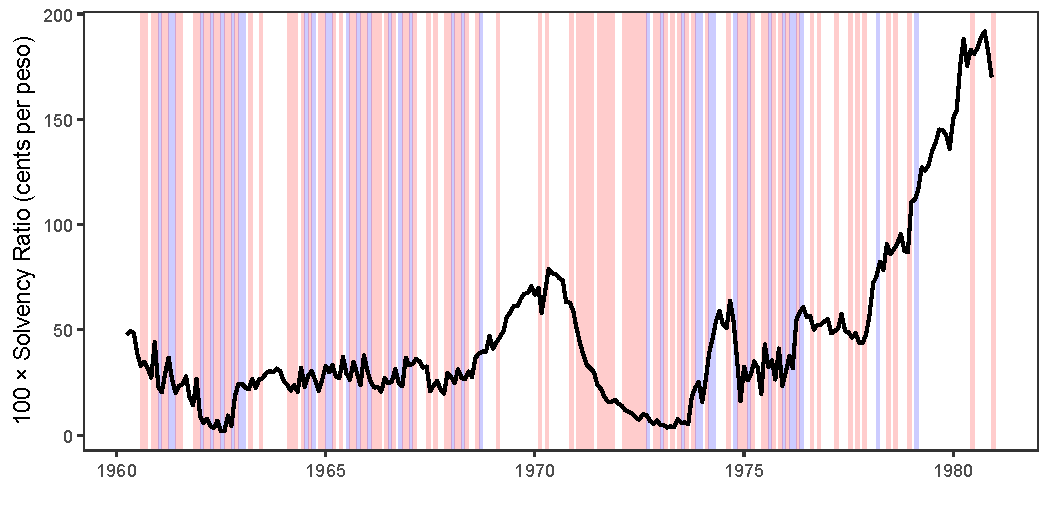
\includegraphics[width=\textwidth]{figures/regime_timeline_level.pdf}
    \caption{Solvency Ratio Stock ($100 \times S_t$)}
    \label{fig:regime_timeline_stock}
\end{subfigure}
\hfill
\begin{subfigure}[b]{0.49\textwidth}
    \centering
    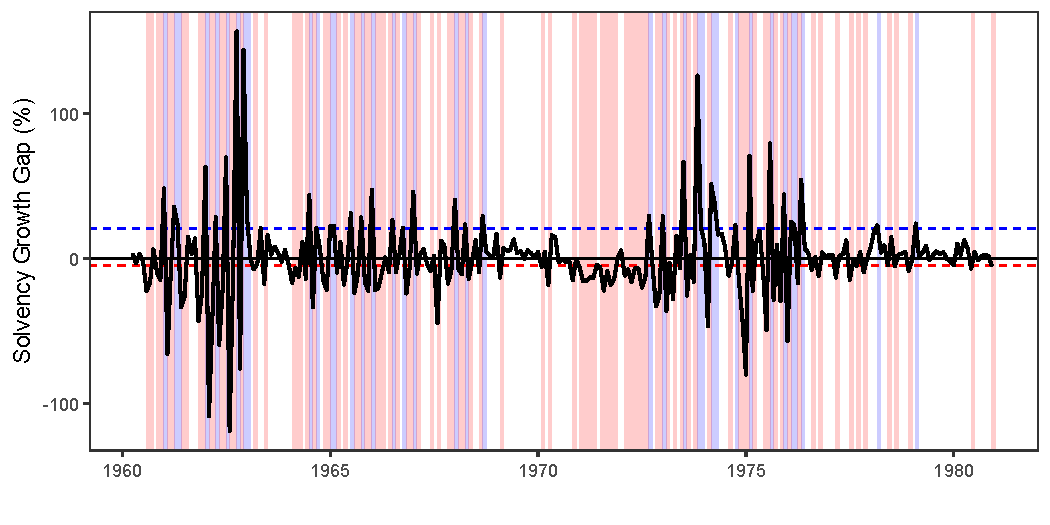
\includegraphics[width=\textwidth]{figures/regime_timeline_gap.pdf}
    \caption{Solvency Growth Gap Flow ($\Delta s_t$)}
    \label{fig:regime_timeline_gap}
\end{subfigure}
\caption{Central Bank Solvency Ratio and Solvency Growth Gap, 1960--1980}
\label{fig:regime_timeline}
\begin{minipage}{\textwidth}
    \vspace{0.3em}
    \footnotesize \textbf{Notes:} \textbf{Panel (A)} displays the monthly Central Bank Solvency Ratio stock ($100 \times S_t \equiv 100 \times [e_t IR_t / (H_t \cdot 1000)]$, expressed as cents per peso). \textbf{Panel (B)} displays the predetermined threshold variable, the Solvency Growth Gap ($\Delta s_t \equiv g^F_t - g^H_t = \Delta \ln S_t \times 100$). Shaded areas distinguish the exploratory three-state diagnostic partition identified by the Concentrated Least Squares grid search: red shading marks the adverse solvency-growth state ($\Delta s_{t-1} \le -4.615\%$, $N=100$), blue shading marks the exploratory upper-tail reserve-accumulation state ($\Delta s_{t-1} > +20.878\%$, $N=38$), and unshaded areas denote the intermediate partition ($N=111$). For econometric estimation and dynamic GIRF simulations, the baseline TVAR pools the two non-adverse partitions into a single unified non-adverse state ($\Delta s_{t-1} > -4.615\%$, $N=145$). The dashed horizontal line in Panel (B) marks the estimated structural threshold ($\hat{\gamma} = -4.615\%$). Data sources: Central Bank of Chile (BCCh) monthly balance sheets (1960:01--1980:12, $N=250$).
\end{minipage}
\end{figure}


\subsubsection{Historical Regime Chronology and the Unidad Popular Trajectory}
\label{sec:tvar_regime_chronology}

\paragraph{Stock-Flow Dynamics: Reserve Exhaustion versus Flow Stabilization.}
The dual-panel trajectory in Figure~\ref{fig:regime_timeline} clarifies the analytical distinction between the level stock of international solvency ($S_t$) and its dynamic flow gap ($\Delta s_t$). Panel~(A) shows that the ratio of official international reserves to Central Bank base money liabilities dropped precipitously in late 1970 and remained near zero throughout 1971--1978. A static stock threshold would classify this entire eight-year window as a single continuous insolvency regime. Such a classification fails to distinguish between active balance-of-payments insolvency and the post-1974 orthodox stabilization under low foreign exchange reserves. Under the military dictatorship, drastic fiscal retrenchment and the contraction of real wages stabilized the flow gap ($\Delta s_t > 0$), despite the depleted stock of reserves.

Panel~(B) demonstrates why the Solvency Growth Gap operates as the true transition trigger. The structural break occurs not when reserve stocks are low in absolute terms, but when base money creation persistently outpaces foreign reserve accumulation. By taking the logarithmic first difference ($\Delta s_t \equiv g^F_t - g^H_t$), the threshold condition $\Delta s_{t-1} \le -4.615\%$ isolates the rate of net reserve depletion. When this gap turns sharply negative, domestic liquidity creation dilutes external reserve backing. The state loses the foreign exchange required to maintain import parities, unanchoring domestic price stability.

\paragraph{Endogenous Dating of the Unidad Popular Macroeconomic Trajectory.}
Without imposing calendar dummies or political intervention dates, the threshold condition $\Delta s_{t-1} \le -4.615\%$ autonomously classifies the critical junctures of the Unidad Popular administration (1970--1973) into the adverse solvency-growth state (reflecting conditions of central-bank insolvency). The mathematical threshold search identifies five distinct historical episodes:
\begin{enumerate}[leftmargin=*,itemsep=1pt]
    \item \emph{November 1970:} Immediate post-electoral capital flight following Salvador Allende's victory triggers an initial gap of $\Delta s_t = -15.18\%$, reflecting commercial bank deposit withdrawals and private asset flight abroad.
    \item \emph{January--May 1971:} The initial redistributive expansion under the Vuskovi\'c Plan drives the growth gap to between $-13\%$ and $-15\%$. High-powered money emission financed public enterprise wage increases while foreign reserves remained stable, initiating the dilution of reserve coverage.
    \item \emph{July--November 1971:} International commercial banks suspended short-term trade credit lines, and US export credit dried up \citep{Stallings1978,DeVylder1976}. The growth gap plunged between $-6\%$ and $-22\%$, reflecting the exhaustion of foreign exchange buffers.
    \item \emph{November--December 1972:} In the aftermath of the October 1972 employer lockout and transport strike \citep[see][]{Casals2021}, the Central Bank extended emergency credit to keep nationalized enterprises operating. The flow gap collapsed to $-26.4\%$ in November and $-33.1\%$ in December.
    \item \emph{February, April, and August 1973:} The final phase of the administration witnessed acute supply bottlenecks for imported spare parts, haul-truck tires, and wheat. With reserves exhausted, the gap reached $-25\%$ to $-36\%$, locking the economy into an accelerating inflation regime.
\end{enumerate}

\paragraph{Endogenous Accommodation versus the Orthodox Narrative of Policy Pathology.}
These empirical findings challenge orthodox accounts of the Chilean transition \citep{DornbuschEdwards1990,Edwards2024}. Mainstream interpretations treat the Unidad Popular inflation as an unforced episode of macroeconomic populism driven by autonomous deficit monetization. In that narrative, monetary policy operates as an independent prime mover unconstrained by external balances. 

The threshold model reveals an alternate institutional mechanism. Monetary emission accelerated defensively to finance enterprise payrolls and purchase essential inputs under strict foreign credit constraints. When foreign commercial banks cut off short-term letters of credit, the state could no longer import intermediate capital goods or food to stabilize domestic markets. Distributive conflict over real income could no longer be pacified through external supply. Under acute reserve depletion, the Central Bank entered an endogenous liquidity accommodation dynamic: price increases required nominal credit expansion to avert enterprise liquidation, which eroded external solvency and amplified inflationary expectations.


\subsubsection{Regime-Dependent Parameter Estimates and Accommodation Dynamics}
\label{sec:tvar_parameter_estimates}

\begin{table}[htbp]
\centering
\small
\renewcommand{\arraystretch}{0.90}
\caption{Regime-Dependent TVAR Parameter Estimates across Solvency Regimes (1960--1980)}
\label{tab:tvar_estimates}
\label{tab:tab04_tvar_estimates}
\resizebox{\textwidth}{!}{%
\begin{tabular}{lccccc}
\toprule
\textbf{Lagged Regressor} & \multicolumn{5}{c}{\textbf{Dependent System Variables ($X_t$)}} \\
\cmidrule(lr){2-6}
 & \textbf{Gold ($g^{gold}_t$)} & \textbf{Imbalance ($\Delta \ln \Theta_t$)} & \textbf{Reserves ($g^F_t$)} & \textbf{Inflation ($\pi_{m,t}$)} & \textbf{Money ($g^H_t$)} \\
\midrule
\multicolumn{6}{l}{\textbf{Panel A: Adverse Solvency-Growth State} ($\Delta s_{t-1} \le -4.615\%$, $N_1 = 100$ months)} \\
\midrule
Constant & 0.636 & -3.720 & 3.388 & -0.300 & 1.893$^{*}$ \\
World Gold Price ($g^{gold}_{t-1}$) & 0.625$^{***}$ & 0.378 & -0.494 & 0.197$^{**}$ & 0.151 \\
Structural Imbalance ($\Delta \ln \Theta_{t-1}$) & --- & -0.188$^{*}$ & --- & 0.010 & --- \\
Reserve Growth ($g^F_{t-1}$) & --- & --- & -0.181 & -0.016 & -0.042 \\
CPI Inflation ($\pi_{m,t-1}$) & --- & --- & 0.512 & 0.684$^{***}$ & 0.581$^{***}$ \\
Base Money Growth ($g^H_{t-1}$) & --- & --- & 0.938 & 0.166$^{***}$ & 0.058 \\
Price Decontrol Dummy ($D_{oct73}$) & -1.225 & 62.520 & 111.026$^{***}$ & 76.213$^{***}$ & -2.775 \\
\midrule
\multicolumn{6}{l}{\textbf{Panel B: Non-Adverse Solvency-Growth State} ($\Delta s_{t-1} > -4.615\%$, $N_2 = 145$ months)} \\
\midrule
Constant & 0.579 & 1.836 & 1.848 & 2.218$^{***}$ & 3.300$^{***}$ \\
World Gold Price ($g^{gold}_{t-1}$) & 0.339$^{***}$ & -1.128$^{**}$ & 0.312 & -0.013 & -0.034 \\
Structural Imbalance ($\Delta \ln \Theta_{t-1}$) & --- & -0.629$^{***}$ & --- & -0.009 & --- \\
Reserve Growth ($g^F_{t-1}$) & --- & --- & -0.355$^{***}$ & -0.014 & 0.006 \\
CPI Inflation ($\pi_{m,t-1}$) & --- & --- & 1.114$^{***}$ & 0.275$^{***}$ & 0.236$^{***}$ \\
Base Money Growth ($g^H_{t-1}$) & --- & --- & -0.173 & 0.240$^{***}$ & 0.115 \\
\bottomrule
\end{tabular}%
}
\begin{minipage}{\textwidth}
\vspace{0.4em}
\footnotesize \textit{Notes:} Monthly series spanning 1960:01--1980:12 ($N=250$, effective sample $T=245$). Conditional Least Squares (CLS) estimates of the five-variable TVAR(1) conditioned on the predetermined Solvency Growth Gap $\Delta s_{t-1} \equiv g^F_{t-1} - g^H_{t-1}$ at the structural threshold $\hat{\gamma} = -4.615\%$. Significance: $^{***} p < 0.01$, $^{**} p < 0.05$, $^{*} p < 0.10$. Dashes (---) denote structural exclusion restrictions: (i) world gold is block exogenous to domestic Chilean variables ($a_{12} = a_{13} = a_{14} = a_{15} = 0$); (ii) real structural imbalance ($\Delta \ln \Theta_t$) is exogenous to domestic feedback ($a_{23} = a_{24} = a_{25} = 0$); and (iii) lagged structural imbalance ($\Delta \ln \Theta_{t-1}$) is excluded from central bank solvency equations ($g^F_t$ and $g^H_t$, $a_{32} = a_{52} = 0$), in accordance with the institutional transmission structure and Latin American structuralist theory. The one-off price decontrol dummy $D_{oct73}$ (Decree Law 522) in Panel A controls for the October 1973 administrative price decontrol and foreign exchange revaluation shock.
\end{minipage}
\end{table}


\paragraph{Equation Estimates and Small-Economy Structural Restrictions.}
Table~\ref{tab:tvar_estimates} reports the conditional least squares parameter estimates for the five-variable Threshold VAR across the adverse solvency-growth state (reflecting conditions of central-bank insolvency) and the non-adverse state. Equation-by-equation estimation isolates the dynamic interactions among world gold prices, the structural import imbalance, international reserves, consumer price inflation, and base money. Following the identification strategy in Section~\ref{sec:tvar_specification}, I impose three structural exclusion restrictions. First, block exogeneity is imposed on the world gold price equation by setting domestic feedback coefficients to zero ($a_{12} = a_{13} = a_{14} = a_{15} = 0$), reflecting Chile's status as a small open economy and price taker in international gold and credit markets; in unrestricted estimations, lagged domestic variables ($\pi_{m,t-1}, g^H_{t-1}, g^F_{t-1}, \Delta \ln \Theta_{t-1}$) are individually and jointly insignificant in the gold equation ($p > 0.10$). Second, domestic feedbacks are excluded from the real structural imbalance equation ($\Delta \ln \Theta_t$), capturing import purchasing capacity constraints as driven by terms of trade and historical import dependence. Third, lagged structural imbalance ($\Delta \ln \Theta_{t-1}$) is excluded from the foreign reserve flow ($g^F_t$) and base money creation ($g^H_t$) equations based on the institutional structure of transmission: structural trade bottlenecks do not mechanically alter reserve flows or print money directly, but operate sequentially through domestic price formation ($\Delta \ln \Theta \to \pi_m$), which the monetary authority accommodates ($\pi_m \to g^H$). Supplementary linear exploratory estimations in Appendix~\ref{app:linear_var_diagnostics} do not provide evidence against this exclusion. In Panel~A, the one-off dummy $D_{oct73}$ controls for the October 1973 administrative price decontrol and foreign exchange revaluation shock under Decree Law 522.

\paragraph{Three Structural Transmission Shifts across Solvency Regimes.}
Comparing parameter estimates across regimes reveals three fundamental structural shifts in the inflation and monetary transmission mechanisms. First, monetary accommodation surges when foreign solvency collapses. In the base money equation ($g^H_t$), the coefficient on lagged inflation ($\pi_{m,t-1}$) rises from $0.236$ ($t = 3.63, p < 0.01$) in the non-adverse state to $0.581$ ($t = 3.90, p < 0.01$) under the adverse solvency-growth state. The accommodation response more than doubles. In the non-adverse state, a 10 percentage point increase in monthly inflation induced only a modest 2.4 percentage point adjustment in base money growth. In the adverse state, that same inflation pulse generated a 5.8 percentage point expansion in base money. When foreign commercial banks canceled short-term credit lines and letters of credit, enterprises could not import replacement machinery or raw materials on deferred payment terms. The Central Bank expanded base money defensively to cover soaring payrolls and working-capital requirements, preventing enterprise illiquidity and factory closures.

Second, price persistence escalates sharply under conditions of central bank insolvency. In the inflation equation ($\pi_{m,t}$), the autoregressive coefficient on lagged inflation rises from $\hat{\beta} = 0.275$ ($t = 6.37, p < 0.01$) in the non-adverse state to $\hat{\beta} = 0.684$ ($t = 8.68, p < 0.01$) in the adverse solvency-growth state. The non-adverse state displays rapid mean reversion. In contrast, the adverse solvency-growth state exhibits near-unit-root inflation inertia. With external reserves depleted, the state could no longer import food or wage goods to stabilize retail prices. Domestic firms engaged in defensive markup revisions, anticipating future currency depreciations and shortages of imported haul-truck tires and spare parts. Speculative hoarding and retail shortages dismantled official price ceilings, cementing self-fulfilling inflation dynamics.

Third, international price pass-through unshields domestic markets during solvency distress. The transmission coefficient from world gold price growth to domestic inflation ($g^{gold}_{t-1} \to \pi_{m,t}$) is economically small and statistically indistinguishable from zero in the non-adverse state ($\hat{\beta} = -0.013, t = -0.23, p = 0.818$). In the adverse solvency-growth state, this pass-through jumps to $\hat{\beta} = +0.197$ ($t = 2.33, p < 0.05$). When foreign exchange reserves are adequate, the Central Bank absorbs external nominal volatility through its reserve buffer and managed import quotas. In the adverse state, this external buffer disintegrates. International monetary instability and US dollar devaluations pass directly into domestic consumer prices through escalating import costs for copper mining equipment and industrial fuels.

\paragraph{Parameter Stability across Threshold Specifications.}
The identified structural shifts remain invariant to the exact placement of the insolvency threshold. The notes to Table~\ref{tab:tvar_estimates} compare the baseline estimates ($\hat{\gamma} = -4.615\%, N_1 = 100$) against the negative-constrained grid search optimum ($\hat{\gamma} = -3.58\%, N_1 = 104$). Across both sample partitions, the key behavioral parameters remain stable. The defensive accommodation coefficient ($\pi_{m,t-1} \to g^H_t$) changes only from $0.581$ to $0.584$ (both $p < 0.01$). Autoregressive inflation persistence shifts from $0.684$ to $0.689$ (both $p < 0.01$). World gold pass-through remains positive and significant ($0.197$ at $p < 0.05$ versus $0.167$ at $p < 0.10$). This parameter stability indicates that the estimated threshold behavior and qualitative regime differences are preserved across alternative threshold locations rather than being driven by local sample sensitivity.



\subsubsection{Dynamic Multipliers and Regime-Dependent Shock Propagation}
\label{sec:tvar_girf_multipliers}

\paragraph{Dynamic Shock Propagation under Endogenous State Transitions.}
To trace how structural shocks propagate dynamically across regimes, the linear impulse response framework must be generalized. In linear vector autoregressions, orthogonalized impulse response functions derived from a Cholesky decomposition assume invariant transmission parameters and history independence. In a Threshold VAR, dynamic propagation depends on the initial state of Central Bank solvency ($\Delta s_{t-1}$), the sign and magnitude of structural innovations to credit or import costs, and the endogenous probability of transitioning across regimes over the forecast horizon.

Following \citet{KoopPesaranPotter1996}, I define the Generalized Impulse Response Function (GIRF) as the expectation of the system's trajectory conditional on a specific structural shock $\nu_t$ and historical information set $\Omega_{t-1}$, relative to an unshocked baseline trajectory:
\begin{equation}
    \text{GIRF}_X(h, \nu_t, \Omega_{t-1}) = \mathbb{E}\left[ X_{t+h} \mid \nu_t, \Omega_{t-1} \right] - \mathbb{E}\left[ X_{t+h} \mid \Omega_{t-1} \right],
    \label{eq:tvar_girf_def}
\end{equation}
where $h = 0, 1, \dots, H$ denotes the forecast horizon. The conditional expectations in Equation~\eqref{eq:tvar_girf_def} are evaluated by Monte Carlo integration. For each regime, I sample $S = 250$ historical starting vectors $\Omega_{t-1}$ belonging to that regime. From each history, the system is simulated forward over $H = 12$ months by drawing $R = 500$ sequences of bootstrap residuals with replacement, preserving empirical non-Gaussianity and contemporaneous residual cross-correlations. In each simulation step, base money growth ($g^H_{t+j}$) and reserve growth ($g^F_{t+j}$) update the endogenous Solvency Growth Gap ($\Delta s_{t+j} \equiv g^F_{t+j} - g^H_{t+j}$), allowing the system to transition endogenously between the adverse solvency-growth state (reflecting conditions of central-bank insolvency) and the non-adverse state.

\paragraph{Evaluating Asymmetric Multipliers across Solvency States.}
To evaluate whether transmission asymmetries between solvency regimes are statistically significant, I formulate a point-wise dynamic multiplier difference test across forecast horizons:
\begin{equation}
    H_0: \Delta_{i,j}(h) \equiv \text{GIRF}_{i,j}^{\text{Insolv}}(h) - \text{GIRF}_{i,j}^{\text{Normal}}(h) = 0,
    \label{eq:tvar_multiplier_diff_test}
\end{equation}
where $\Delta_{i,j}(h)$ measures the difference in the dynamic response of variable $i$ to a structural shock in variable $j$ between the adverse solvency-growth state (reflecting conditions of central-bank insolvency) and the non-adverse state at horizon $h$. Confidence intervals (90\% and 95\%) for the multiplier differences are computed via the percentile bootstrap across the resampled histories. The complete set of 16 empirical impulse response pathways, dynamic multiplier difference tests across all 25 shock-response pairs, and endogenous regime-switching probability matrices are documented in Appendix~\ref{app:tvar_girf_atlas}.

\paragraph{Forward Transmission versus Reverse Accommodation: Dynamic Multiplier Analysis.}
Contrasting the speed, scale, and persistence of forward versus reverse transmission directly evaluates the central theoretical dispute of this chapter. Orthodox accounts \citep{DornbuschEdwards1990,Edwards2024} argue that discretionary high-powered money creation functioned as the primary autonomous driver of the Chilean inflation. The dynamic Generalized Impulse Response trajectories in Figure~\ref{fig:tvar_girf_tournament} are difficult to reconcile with that premise. 

Forward monetary transmission ($g^H \to \pi_m$, Panel~A) operates with modest magnitude and gradual momentum. In the adverse solvency-growth state (reflecting conditions of central-bank insolvency), a one-standard-deviation innovation to base money growth increases monthly consumer price inflation by a peak of $0.966$ percentage points at month 1 ($h=1$). Statistical significance persists across nine consecutive months ($h=1$ to $9$), generating a cumulative price acceleration of $3.550$ percentage points over the year. In the non-adverse solvency-growth state, the response peaks at $1.256$ percentage points at month 1 and remains significant for six months ($h=1$ to $6$), with a cumulative expansion of $2.215$ percentage points. The dynamic multiplier difference ($\Delta_{g^H \to \pi_m}(h)$) is statistically significant across months 4 through 8, peaking at $+0.313$ percentage points at month 3. Forward transmission operates with measurable persistence, but its response profile is constrained. High-powered money emission does not induce an instantaneous hyperinflationary explosion.

\begin{figure}[htbp]
\centering
\begin{subfigure}[b]{0.49\textwidth}
    \centering
    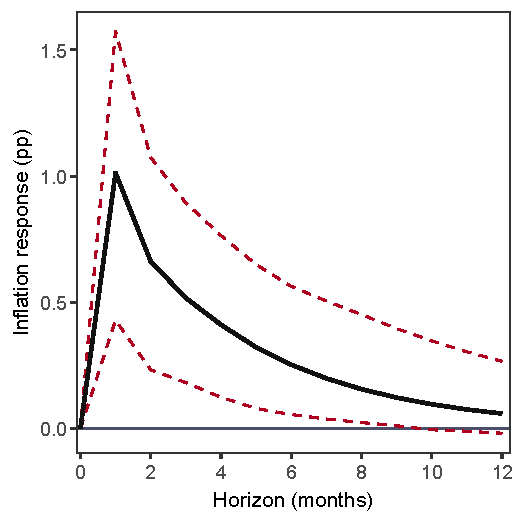
\includegraphics[width=\textwidth]{figures/tvar_girf_forward_money.pdf}
    \caption{Forward Monetary Transmission ($g^H \to \pi_m$)}
    \label{fig:tvar_girf_forward_money}
\end{subfigure}
\hfill
\begin{subfigure}[b]{0.49\textwidth}
    \centering
    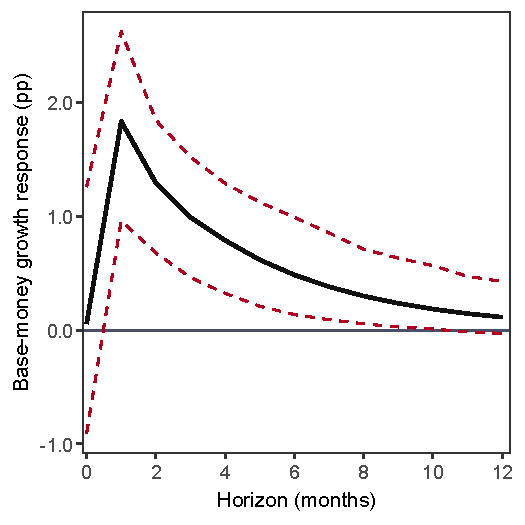
\includegraphics[width=\textwidth]{figures/tvar_girf_reverse_accom.pdf}
    \caption{Reverse Accommodation ($\pi_m \to g^H$)}
    \label{fig:tvar_girf_reverse_accom}
\end{subfigure}
\caption{Dynamic Multipliers under Adverse Solvency-Growth Conditions: Forward Transmission versus Reverse Accommodation}
\label{fig:tvar_girf_tournament}
\begin{minipage}{\textwidth}
    \vspace{0.3em}
    \footnotesize \textbf{Notes:} Generalized Impulse Response Functions (GIRFs) over a 12-month horizon in the adverse solvency-growth state ($\Delta s_{t-1} \le -4.615\%$, reflecting conditions of central-bank insolvency). Solid black lines trace median bootstrap responses to a one-standard-deviation structural innovation; dashed crimson lines represent 90\% empirical bootstrap confidence bands derived from 500 outer bootstrap replications and 1,000 inner Monte Carlo draws. The horizontal benchmark line marks zero. \textbf{Panel (A)} displays forward monetary transmission from Central Bank base money expansion to consumer price inflation ($g^H \to \pi_m$). \textbf{Panel (B)} displays reverse accommodation from consumer price inflation to base money growth ($\pi_m \to g^H$).
\end{minipage}
\end{figure}

In sharp contrast, reverse accommodation ($\pi_m \to g^H$, Panel~B) is more persistent and larger in cumulative magnitude over the reported horizon than forward transmission; the point-wise difference is statistically significant from months 2 through 10. In the adverse solvency-growth state, an unexpected price shock induces an immediate acceleration in base money growth that peaks at $1.715$ percentage points at month 1 ($h=1$) and sustains unbroken statistical significance across 10 consecutive months ($h=1$ to $10$). Over the 12-month horizon, this defensive monetization injects $6.537$ percentage points of cumulative high-powered money. The point-wise multiplier difference ($\Delta_{\pi_m \to g^H}(h)$) is strictly positive and statistically significant across nine consecutive months ($h=2$ to $10$), peaking at $+0.837$ percentage points at month 2. In both initial impact and cumulative volume ($6.54$ pp versus $3.55$ pp), reverse accommodation outstrips forward monetary transmission. Prices drag base money behind them far more aggressively than base money pushes prices forward.

This asymmetry captures the institutional reality of the Unidad Popular period. Following the October 1972 employer lockout and transport strike \citep{Casals2021}, commercial trade credit lines froze and inventories accumulated in nationalized enterprises. To prevent production halts, enterprise illiquidity, and payroll defaults across hundreds of thousands of workers, the Central Bank expanded the discount window defensively. Base money growth was the consequence of real bottlenecks and distributive conflict, not an autonomous monetary experiment.

\paragraph{The Dissolution of the External Buffer: World Price Pass-Through.}
Figure~\ref{fig:tvar_girf_gold_shield} illustrates the external balance-of-payments constraint facing a financially dependent economy. In the non-adverse state (Panel~A), when Central Bank foreign exchange reserves are adequate, a one-standard-deviation world gold price shock produces zero statistically significant impact on domestic inflation at any horizon ($h=0$ to $12$). The peak response is $0.210$ percentage points at month 1, and the 90\% confidence interval encompasses zero throughout the year. Convertible reserves act as an external buffer: the Central Bank absorbs international monetary turbulence through foreign exchange settlements and managed import allocations.

\begin{figure}[htbp]
\centering
\begin{subfigure}[b]{0.49\textwidth}
    \centering
    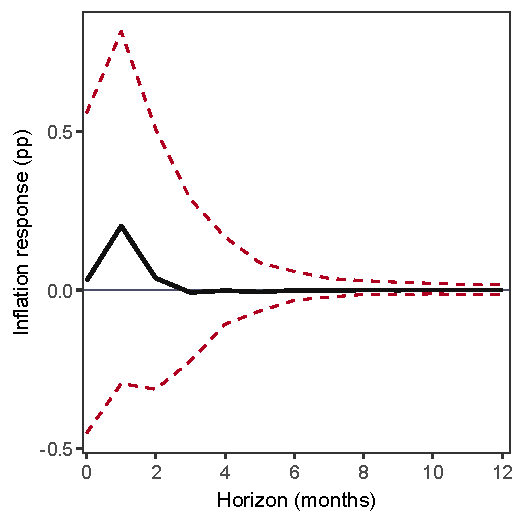
\includegraphics[width=\textwidth]{figures/tvar_girf_gold_normal.pdf}
    \caption{Non-Adverse Solvency-Growth State ($\Delta s_{t-1} > -4.615\%$)}
    \label{fig:tvar_girf_gold_normal}
\end{subfigure}
\hfill
\begin{subfigure}[b]{0.49\textwidth}
    \centering
    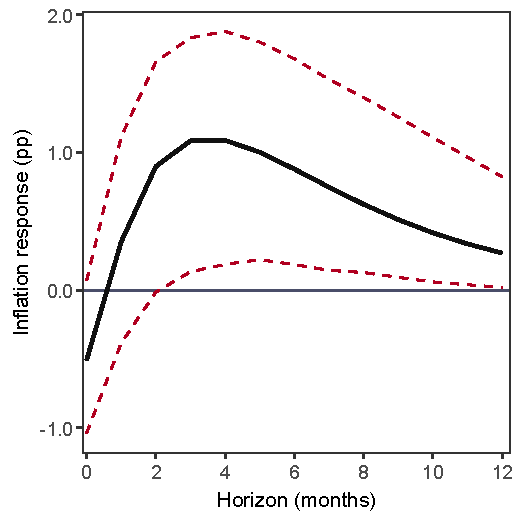
\includegraphics[width=\textwidth]{figures/tvar_girf_gold_insolv.pdf}
    \caption{Adverse Solvency-Growth State ($\Delta s_{t-1} \le -4.615\%$)}
    \label{fig:tvar_girf_gold_insolv}
\end{subfigure}
\caption{International Price Pass-Through across Solvency Regimes: The Dissolution of the External Buffer}
\label{fig:tvar_girf_gold_shield}
\begin{minipage}{\textwidth}
    \vspace{0.3em}
    \footnotesize \textbf{Notes:} Generalized Impulse Response Functions (GIRFs) of domestic consumer price inflation ($\pi_m$) to a one-standard-deviation structural shock in world gold price growth ($g^{gold}$) across solvency states. Solid black lines trace median bootstrap responses; dashed crimson lines represent 90\% empirical bootstrap confidence bands derived from 500 outer bootstrap replications and 1,000 inner Monte Carlo draws. The horizontal benchmark line marks zero. \textbf{Panel (A)} displays transmission in the non-adverse state ($\Delta s_{t-1} > -4.615\%$). \textbf{Panel (B)} displays transmission in the adverse solvency-growth state ($\Delta s_{t-1} \le -4.615\%$), reflecting conditions of central-bank insolvency.
\end{minipage}
\end{figure}

In the adverse solvency-growth state ($\Delta s_{t-1} \le -4.615\%$, Panel~B, reflecting conditions of central-bank insolvency), this insulation mechanism dissolves. The identical international price shock unleashes an unbroken 10-month inflationary wave ($h=3$ to $12$). Domestic inflation accelerates to a peak of $0.982$ percentage points at month 3 and delivers a cumulative price expansion of $6.542$ percentage points. The point-wise multiplier difference test ($\Delta_{g^{gold} \to \pi_m}(h)$) is strictly positive and statistically significant across all 10 consecutive months ($h=3$ to $12$), peaking at $+0.999$ percentage points at month 3. Adequate foreign reserves insulate the domestic economy; depleted reserves leave it vulnerable to international price shocks. When external commercial credit dried up and liquid reserves fell near zero, the state could no longer convert domestic currency into world money to stabilize import costs. International inflation transmitted directly into domestic consumer prices.

\paragraph{Cost-Push Inflation Inertia and Structural Imbalance Magnification.}
The non-linear transmission dynamics extend to domestic price persistence and real structural trade imbalances. In the non-adverse state, an unexpected domestic price shock ($\pi_m \to \pi_m$) accelerates monthly inflation by $3.786$ percentage points on impact, but dissipates steadily, losing statistical significance by month 7 with a cumulative effect of $6.459$ percentage points. In the adverse solvency-growth state, price momentum locks into the system: statistical significance persists across 11 consecutive months ($h=0$ to $10$), generating nearly double the cumulative price acceleration ($11.655$ percentage points). The persistence differential ($\Delta_{\pi_m \to \pi_m}(h)$) peaks at $+1.048$ percentage points at month 2 and maintains unbroken statistical significance for nine consecutive months ($h=2$ to $10$). In non-adverse periods, the state can damp distributive conflict by importing wage goods; under solvency distress, the inability to import turns every price shock into an entrenched markup struggle.

Real structural trade imbalance shocks ($\Delta\ln\Theta \to \Delta\ln\Theta$) likewise propagate asymmetrically. In the non-adverse state, the import-export gap displays monotonic decay ($+39.667$ percentage points on impact, cumulative $+24.523$ percentage points). In the adverse solvency-growth state, the initial imbalance ($+45.674$ percentage points) triggers an amplified oscillatory cycle. The regime differential peaks at $+15.364$ percentage points at month 1 and remains statistically significant across nine consecutive months ($h=1$ to $9$). Balance-of-payments distress destabilizes the physical import pipeline, creating recurring shortages of haul-truck tires, industrial replacement parts, and agricultural inputs rather than a smooth real adjustment. Finally, simulated regime-switching probabilities indicate that crossing between states is not driven by isolated monthly shocks: from the non-adverse state, the probability shift of crossing into the adverse state is negligible ($\Delta P \approx 0$). Once the system is in the adverse solvency-growth state ($\Delta s_{t-1} \le -4.615\%$, reflecting conditions of central-bank insolvency), favorable terms-of-trade shocks also produce negligible probability changes ($\Delta P \approx 0$). The simulated probability changes are negligible under these shocks, indicating persistence of the fitted adverse state over the reported horizon.



\subsubsection{Synthesis: Non-Linearity and the Peripheral Monetary Circuit}
\label{sec:tvar_synthesis}

\paragraph{Resolving the Nominal Paradox: Money as Consequence, Not Prime Mover.}
The regime-dependent parameter estimates resolve the central empirical puzzle of the Chilean inflation. Orthodox accounts treat the statistical correlation between base money growth and consumer price inflation during 1972--1973 as proof of an exogenous, printing-press-driven inflationary breakdown. Within the identified TVAR, the estimated response from inflation to base-money growth is more persistent and cumulatively larger under insolvency than the reverse response, more consistent with a substantial accommodation channel than with a purely autonomous-money interpretation. In the non-adverse state, base money growth accommodates inflation only modestly ($\hat{\beta} = 0.24$). In the adverse solvency-growth state ($\Delta s_{t-1} \le -4.615\%$, reflecting conditions of central-bank insolvency), accommodation surges to $\hat{\beta} = 0.58$ and inflation persistence jumps to $0.68$. The high observed correlation between money and prices reflects an endogenous consequence of structural solvency distress. The Central Bank expanded domestic liquidity to finance enterprise payrolls and prevent immediate liquidation, even as external supply ceased.

\paragraph{The Peripheral Monetary Circuit and the Hard-Currency Ceiling.}
These threshold dynamics illustrate the material limits of the peripheral monetary circuit. In an asymmetric international currency hierarchy, the state can issue domestic fiat liabilities, but it cannot manufacture world money. When foreign trade credit lines were severed and liquid reserves drained toward zero, the state could no longer convert domestic base money into essential imported machinery, spare parts, or food. Distributive conflict over real income could no longer be dampened through external supply. Under acute solvency depletion, domestic credit expansion dilutes external backing, leaving international price shocks unbuffered, generating persistent inflationary pressure, and inducing defensive monetization.

\paragraph{From Reserve Balance Sheets to the Political Economy of Subordination.}
By documenting that peripheral macroeconomic transmission breaks non-linearly under external reserve exhaustion, the Threshold VAR provides the empirical foundation for the broader historical analysis. Section~\ref{sec:discussion_conclusion} builds upon these findings to evaluate the political economy of the international credit blockade, organized distribution sabotage, and the institutional limits of peripheral monetary sovereignty.



